\documentclass[11pt,a4paper,oldfontcommands]{memoir}
\usepackage[utf8]{inputenc}
\usepackage[T1]{fontenc}
\usepackage{microtype}
\usepackage[dvips]{graphicx}
\usepackage{graphicx}
\usepackage{caption}
\usepackage{subcaption}
\usepackage{xcolor}
\usepackage{times}


\graphicspath{ {figures/} }
\usepackage{array}

\usepackage[french]{babel}
\usepackage{layout}
\usepackage{verbatim}[4]
\usepackage{color}

\usepackage{titlesec}
\usepackage{verbatim}
\usepackage{listings}
\usepackage{ulem}

\setcounter{secnumdepth}{4}

\titleformat{\paragraph}
{\normalfont\normalsize\bfseries}{\theparagraph}{1em}{}
\titlespacing*{\paragraph}
{0pt}{3.25ex plus 1ex minus .2ex}{1.5ex plus .2ex}

\usepackage[
breaklinks=true,colorlinks=true,
%linkcolor=blue,urlcolor=blue,citecolor=blue,% PDF VIEW
linkcolor=black,urlcolor=black,citecolor=black,% PRINT
bookmarks=true,bookmarksopenlevel=2]{hyperref}

\usepackage{geometry}
% PDF VIEW
% \geometry{total={210mm,297mm},
% left=25mm,right=25mm,%
% bindingoffset=0mm, top=25mm,bottom=25mm}
% PRINT
\geometry{total={210mm,297mm},
left=25mm,right=25mm,
bindingoffset=10mm, top=25mm,bottom=25mm}

\OnehalfSpacing
%\linespread{1.3}

%%% CHAPTER'S STYLE
%\chapterstyle{bianchi}
\chapterstyle{ger}
%\chapterstyle{madsen}
%\chapterstyle{ell}
%%% STYLE OF SECTIONS, SUBSECTIONS, AND SUBSUBSECTIONS
\setsecheadstyle{\Large\bfseries\sffamily\raggedright}
\setsubsecheadstyle{\large\bfseries\sffamily\raggedright}
\setsubsubsecheadstyle{\bfseries\sffamily\raggedright}


%%% STYLE OF PAGES NUMBERING
%\pagestyle{companion}\nouppercaseheads
%\pagestyle{headings}
%\pagestyle{Ruled}
\pagestyle{plain}
\makepagestyle{plain}
\makeevenfoot{plain}{\thepage}{}{}
\makeoddfoot{plain}{}{}{\thepage}
\makeevenhead{plain}{}{}{}
\makeoddhead{plain}{}{}{}


\maxsecnumdepth{subsection} % chapters, sections, and subsections are numbered
\maxtocdepth{subsection} % chapters, sections, and subsections are in the Table of Contents


%%%---%%%---%%%---%%%---%%%---%%%---%%%---%%%---%%%---%%%---%%%---%%%---%%%

\begin{document}

%%%---%%%---%%%---%%%---%%%---%%%---%%%---%%%---%%%---%%%---%%%---%%%---%%%
%   TITLEPAGE
%
%   due to variety of titlepage schemes it is probably better to make titlepage manually
%
%%%---%%%---%%%---%%%---%%%---%%%---%%%---%%%---%%%---%%%---%%%---%%%---%%%
\thispagestyle{empty}

{%%%
\sffamily
\centering
\Large

~\vspace{\fill}

{\huge
Tenter la \textit{Fake News Challenge}.\\
{\LARGE
Une proposition d'utilisation de la \textit{Stance Detection} pour mieux anticiper le phènomène des \textit{Fake News}.
}
}

\vspace{2.5cm}

{\LARGE
 Enzo POGGIO
}

\vspace{3.5cm}

Ce mémoire est le travail final du\\
Master d'informatique pour sciences humaines\\[1em]
de la\\[1em]
Faculté des Lettres\\
Université de Genève

\vspace{3.5cm}

Superviseuse: Professeure Paola Merlo

\vspace{\fill}

Mai 2018

%%%
}%%%

\cleardoublepage
%%%---%%%---%%%---%%%---%%%---%%%---%%%---%%%---%%%---%%%---%%%---%%%---%%%
%%%---%%%---%%%---%%%---%%%---%%%---%%%---%%%---%%%---%%%---%%%---%%%---%%%

\tableofcontents*


\clearpage

%%%---%%%---%%%---%%%---%%%---%%%---%%%---%%%---%%%---%%%---%%%---%%%---%%%
%%%---%%%---%%%---%%%---%%%---%%%---%%%---%%%---%%%---%%%---%%%---%%%---%%%
\chapter{Introduction: Qu'est-ce qu'une \textit{Fake News}?}


Lors des voeux annuels présidentiels de 2018 en France,  \href{https://www.20minutes.fr/politique/2196019-20180103-vux-presse-macron-veut-censurer-fake-news-prone-saine-distance-entre-pouvoir-medias}{« Emmanuel Macron s’est trouvé un ennemi commun avec les médias : la lutte contre les fausses nouvelles, ou \textit{Fake News} comme le disent les Anglo-saxons»}.
Le but du président est de sanctionner juridiquement les fausses nouvelles et les maux qu'elles engendrent.
Le but second est de portéger la vie démocratique, surtout en période d'éléction.
Donné un définition légal aux fausses nouvelles nous interroge sur leur nature.
Dans le sens commun ou par l'usage, la fausses nouvelles est «tous ce que je ne suis pas d'accord avec».
On voit tout de suite les limites de ce type de définition.
Deux personnes avec des opinions contraire traiteraient les informations de l'autre comme des fausses nouvelles.
Alors comment faut-il faire ?
Y a-t-il un bonne définiton des fausses nouvrelles (\textit{Fake News}) ?
Peut-on parler de \textit{Fake News} de manière objective ?
Qu'implique le terme \textit{Fake News} ?
D'ou proviennent ces fameuses \textit{Fake News} et que font-elles ?
Et pourquoi est-ce important d'en parler ?

Nous répondrons à ces questions en présentant dans cette partie notre définition des \textit{Fake News}, leurs raisons d'être, leurs provenances, leurs moyens de propagation et les risques qu'elles entrainent.
Puis enfin nous présenterons un moyen pour les détecter.


\section{Vers une définition du concept de \textit{Fake News}.}

\subsection{Produire des \textit{Fake News}; une intention de tromper.}
Un énoncé peut être vrai ou faux.
Il est vrai : s'il est en adéquation avec le monde.
Il est faux : s'il ne correspond pas à la réalité.
Les nouvelles (news) sont des énoncés.
Est-ce que l'énoncé « J'aime les tartes. »  est une news ?
Non, toutes les news sont des énoncés; mais seul certains énoncés sont des news. Des journalistes ont fait une liste non exhaustive des critères d'une news (\href{http://www.tandfonline.com/doi/full/10.1080/1461670X.2016.1150193}{Tony Harcup et Deirdre O’Neill, 2016}).
La news est une histoire d'une personne de pouvoir ou célèbre.
\textit{\href{https://www.francebleu.fr/infos/medias-people/le-chanteur-johnny-hallyday-est-mort-1512527631}{«Concert annulé de Bertrand Cantat [...]»}}
Elle est parfois une bonne ou une mauvaise nouvelle.
\textit{\href{https://www.voici.fr/news-people/actu-people/concert-annule-de-bertrand-cantat-des-associations-comptaient-manifester-dans-lolympia-646342}{«Johnny Hallyday est mort à l'âge de 74 ans»}}.
Souvent elle est une surprise ou un phénomène qui concerne beaucoup de personnes.
\href{}{«\textit{Ouragan Maria. L’état de catastrophe naturelle} [déclaré ...]»}.
Certaines sont juste des suivis.
\textit{\href{https://blogs.mediapart.fr/rachid-barbouch/blog/230318/accusations-contre-mediapart-edwy-plenel-repond-nicolas-sarkozy}{«Accusations contre Médiapart : Edwy Plenel répond à Nicolas Sarkozy »}}.
Et parfois ce sont juste des divertissements ou des faits divers.
\textit{\href{http://www.purepeople.com/article/alexia-mori-enceinte-elle-devoile-combien-de-kilos-elle-a-pris_a284197/1}{«Alexia Mori enceinte : Elle dévoile combien de kilos elle a pris !»}}.
En somme, retenons qu'une nouvelle est une histoire en lien avec la réalité.
Ce qui nous intéresse c'est sa véracité selon l'interprétation du monde réel.
Cependant, leurs sujets sont variés, mais ce n'est pas pertinent pour nous.
De manière, plus générale une nouvelle est une histoire relayée par un média.
Les médias de communication des news sont pluriels.
Pour les citer de manière non-exhaustives, nous avons: la presse papier, la télévision, les radio-fréquences et les réseaux-sociaux (facebook, twitter, etc.).

L'erreur est une opinion, un jugement ou une information non conforme avec la réalité ou la vérité.
Imaginons qu' un individu pense et déclare que: tous les cygnes sont blancs et que toutes les personnes racisés volent.
Cet individu se trompe car il existe des cygnes noir et des personnes racisés qui n'ont jamais volé de leur vie.
L'erreur est inconsciente.
Elle n'est pas faite exprès.
Celle-ci démasquée, elle tend à être corrigée. Imaginons qu'un journal, par inattention, présente un photo qui ne correspond pas au sujet de sa chronique.
Le journal publiera par la suite un
\textit{\href{http://www.leparisien.fr/culture-loisirs/erratum-06-11-2016-6294522.php}{«Erratum»}}.
Une nouvelle erronée est donc une histoire médiatisée qui n'est pas vraie.
Elle ne correspond pas à la vérité.
La nouvelle erronée est due à une erreur scientifique ou bien une erreur journalistique.
C'est-à-dire une mauvaise manipulation de l'information par l'un de ces deux corps.
Les médias précautionneux corrigent leurs nouvelles erronées par des articles de démenti.
Ceci devrait être le code de déontologie des journalistes pour l'honnêteté intellectuelle.
Une \textit{Fake News}\footnote{En français, nouvelle truquée mais le terme \textit{Fake News} est devenu tellement commun
 en français qu'il sera utilisé dans ce mémoire.} n'est pas une nouvelle erronée.
Cependant elles sont souvent confondues.

Parfois des nouvelles sont volontairement erronées.
On dit alors qu'elles sont fausses.
Il faut distinguer deux types de fausses nouvelles.
Le point important ici est l'intention derrière.

Les fausses nouvelles dans un but bien-veillant s'appellent satire ou information parodique.
Ces parodies imitent les médias.
Ils volent même jusqu'à leur nom parfois (le Gorafi est l'anagramme du Figaro).
Mais au lieu de diffuser de vraies informations, les parodies proposent un contenu décalé, sarcastique ou canularesque.
Le but premier de ce genre de nouvelle est le divertissement.
\href{http://www.legorafi.fr/2018/03/28/heritage-de-stephen-hawking-sa-famille-se-dispute-pour-savoir-qui-obtiendra-le-trou-noir-dans-son-garage/}{«Héritage de Stephen Hawking : Sa famille se dispute pour savoir qui obtiendra le trou noir dans son garage»}.
\href{http://www.bilboquet-magazine.fr/barilla-doliprane-lancent-pates-speciales-fin-soiree-vrais-morceaux-daspirine/}{«Barilla et Doliprane lancent des pâtes spéciales « fin de soirée » avec des vrais morceaux d’aspirine»}.
Même si l'on trompe le lecteur, on ne cherche pas à lui nuire mais plutôt à le faire rire.
Enfin il y a toujours des exceptions où l'information semble tellement crédible qu'elle est ensuite utilisée comme source fiable. \href{http://leplus.nouvelobs.com/contribution/1141462-christine-boutin-cite-le-gorafi-sur-bfmtv-si-j-etais-pro-manif-pour-tous-j-aurais-honte.html}{«Christine Boutin cite Le Gorafi sur BFMTV [...]»}
Les parodies donnent des informations délibérément fausses.
La tromperie est totalement assumée et même souvent revendiquée.

Les fausses nouvelles dans le but de volontairement tromper sont ce que l'on appelle \textit{Fake News}.
Elle se distingue de l'erreur car elle n'est pas le produit du hasard ou d'une mauvaise manipulation.
Et elle se distingue de la satire et de la parodie car elle n'est ni assumée ni revendiquée fausse.
La \textit{Fake News} provient d'une personne s'exprimant publiquement ou d'un ensemble de médias.
Elle participe à la désinformation via les médias et les réseaux sociaux.
Souvent, les \textit{Fake News} sont écrites par des anonymes difficilement contestables et calomniables.

Pour prendre un site parmi tant d'autre, \href{http://secretnews.fr/}{Secretnews} est un site colportant des fausses informations par exemple :
\href{http://secretnews.fr/2017/06/18/alain-finkielkraut-a-mort-leguerai-patrimoine-aux-migrants/}{«Alain Finkielkraut : « À ma mort, je léguerai tout mon patrimoine aux migrants.»».}
Or monsieur Finkielkraut n'a pas rédiger son testament pour les migrants.
Il est dit dans cette article que monsieur Finkielkraut aurait dans un  interview au Figaro exprimer son souhait de léguer son patrimoine immobilier à la France à des fins de logement pour les migrants.
Mais il n'existe aucune trace du dit article.
Bien sur cette information n'a pas d'auteur autre que le site qui ne donne aucun contact.
Le site revendique que «toutes \sout{nos} [leur] sources sont vérifiées par un huissier assermenté».
Mais aucun rapport ou mandat de justice n'est donné.
Les informations sur cette page paraissent tellement folles que l'on pourait se demander s'il ne s'agit pas d'une satire.

Pendant l'\href{https://www.youtube.com/watch?v=uCPuiSWRq8I}{«Émission politique»} diffuser le 3 novembre sur la chaîne publique france 2, Jean-luc Mélenchon fait plusieurs affirmations qui sont controversées.
Il dit premièrement que la France à le record des millionnaires.
Or cette information est fausse d'après l'étude du capgemini le \href{https://www.worldwealthreport.com/download}{«World Wealth Report 2017»}.
Ensuite il nie que l'opposition vénézuelienne se serait fait frapper devant leur assemblée le 5 juillet 2017 alors que des médias vénézuelien comme \textit{Noticias RCN} on partageait des \href{https://www.noticiasrcn.com/internacional-crisis-venezuela/seguidores-chavistas-irrumpen-violencia-asamblea-nacional}{vidéos} de la répression qui a eu lieu.
Il défend ici dans l'interview d'autres arguments en faveur du gouvernement de Maduro.
Mais la plupart sont factuellement faux.
Ici Jean-Luc Mélenchon répend des \textit{Fake News}.

Le 29 mars 2018 le site Direct Actu partage un photo qui fait polémique sur plusieurs médias peu scrupuleux.
Il titre à cette photo \href{http://www.directactu.net/2018/03/29/un-politicien-bresilien-corrompu-accroche-a-un-poteau/}{«Un politicien brésilien corrompu accroché à un poteau !»}.
Une citation de l'article dit : «Marcionólio da Costa Mendes a été attaché à un poteau par la population de Mata Grande, dans l’État de Alagoas. Accusé d’avoir volé dans les caisses publiques, le parlementaire a été innocenté par le tribunal de justice, ce qui a provoqué la colère des habitants de la commune.».
Le fond de l'article reste à vérifier mais en tout cas la photo partager n'est pas celle de Marcionólio da Costa Mendes.
Premièrement le visage du personnage est brouillé donc pas de reconnaissance.
Deuxièmement la photo est celle d'une publicité pour une banque australienne : \href{https://thefinancialbrand.com/19014/nab-guerilla-marketing-stunts/}{The financial brand}.

\begin{center}
 \begin{figure}[h]
  \begin{subfigure}{.5\textwidth}
   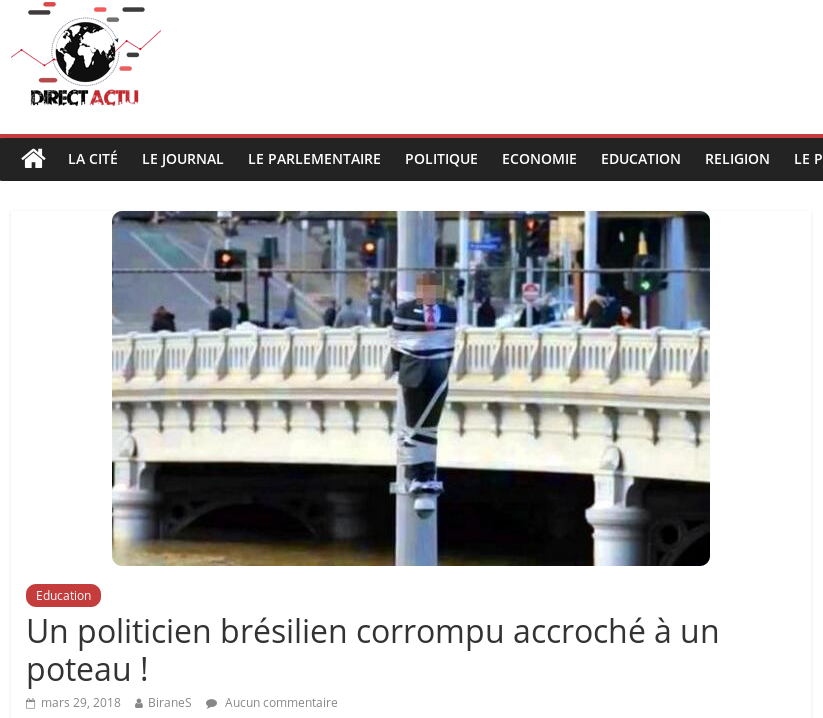
\includegraphics[scale=0.240]{../../img/directactu.png}
   \caption{Un politicien brésilien corrompu accroché à un poteau !}
   \label{brezil}
  \end{subfigure}
  \begin{subfigure}{.5\textwidth}
   
\includegraphics[scale=0.250]{../../img/financialbrand.png}
   \caption{Doug Gets Tied to a Pole}
   \label{financialbrand}
  \end{subfigure}
  \caption{Une photo servant à une campagne publicitaire et à une \textit{Fake News}}
  \label{compafaketruth1}
 \end{figure}
\end{center}

Ici Direct Actu partage un fausse information la photo de l'article ne correspond pas à la réalité qui y est décrite.

\subsection{Limites de la définition.}
Certes une erreur peut arriver dans le traitement ou la création de l'information.
Mais ces erreurs sont-elles légitimes ?
La science progresse en faisant des erreurs.
D'ailleurs, dans la définition de l'étude scientifique l'erreur joue un rôle important.
L'étude scientifique est la recherche perpétuelle de l'erreur.
À défaut de nous apprendre ce qu'est la vérité, la science nous montre ce qu'elle n'est pas.
Donc l'erreur scientifique est légitime au bon fonctionnement de la science.
Peut-on en dire autant de l'erreur journalistique ?
Le journaliste doit faire un compte rendu exhaustif, objectif et vraisemblable du sujet qu'il traite.
Si une erreur non scientifique vient se faufiler dans son article c'est qu'il a mal fait son travail.

Par exemple, on voit toujours des médias relayer l'information que les vaccins causent l'autisme chez l'enfant.
Cette croyance persiste après une publication d'Andrew Wakefield
\footnote{Andrew Wakefield est un ancien chirurgien britannique et chercheur médical connu pour ses prétentions frauduleuses entre le vacin ROR et l'autisme.
 Il fut radié de l'ordre des médecins en mai 2010 pour défaut à son devoir de consultant responsable.}.
Cette publication fut démentie des centaines de fois par des autorités compétentes, mais les médias de grande audience relayent toujours ce message de méfiance vaccinale.
Le devoir du journaliste n'est alors pas respecter .
Les médias traditionnels entretiennent le discours erroné des antivax
\footnote{Partisans de la controverse sur la vaccination qui remet en cause son efficacité et la sécurité de certains vaccins.}.
Celui-ci fait s'écouler beaucoup d'encre.
Mais cette controverse est de la désinformation pure et d'une grande malhonnêteté intellectuelle. On retrouve sur le site de fausses informations StopMensonge, cet article: \href{https://stopmensonges.com/le-president-duterte-banni-les-vaccins-aux-philippines-les-vaccinations-provoquent-lautisme/}{«Le Président Duterte banni les vaccins aux Philippines: « Les Vaccinations provoquent l’Autisme »»}.
Certainement que l'informations est totalement fausses;  les Philippines aussi utilisent la technologies des vaccins.
Mais cela est fait pour donner un doute au lecteur sur la vaccination.
Et après quand les médias de hautes audience comme FranceInfo publie un article :
\href{https://www.francetvinfo.fr/sante/vaccins/vaccination-et-autisme-nous-reclamons-justice-et-reparation-pour-nos-enfants-blesses-par-leur-vaccin_2297901.html}{«Vaccination et autisme : Nous réclamons justice et réparation pour nos enfants blessés par leur vaccin»}. les indécis qui avaient lu des articles comme celui de StopMensonge croient en cette désinformation persistante malgré les méta-analyses qui sont négatives sur ce lien de causalité.
Les médias sont toujours le vecteurs de transmissions de cette \textit{Fake News}.

\section{Pourquoi produire des \textit{Fake News}?}

\subsection{Le contexte des \textit{Fake News}.}
%Dans une presse de plus en plus virtualisée chacun peut devenir l'auteur d'un article.
L'invention qui a le plus contribué à l'essor des médias est certainement l'imprimerie.
Elle nous fait passer des histoires orales à la presse.
L'information est figée sur du papier.
Elle n'est plus perdue ou transformée par le locuteur de l'histoire.
À partir de ces documents, on peut faire des versions officielles et approuvées par une autorité.
L'information fut pendant très longtemps partagée de manière verticale.
La source d'autorité de la connaissance était plus ou moins légitime et compétente.
La connaissance était donnée par les médias et leur vision. Il n'y avait pas de sources contestataires.

Puis fut créé internet ! Internet permet un partage des connaissances horizontal.
Tout le monde disposant d'une connexion au réseau peut participer à la connaissance générale.
Chacun peut écrire, partager et relayer des informations.
Les médias se sont développé sur internet et surtout ils s'y sont multipliés.
La pluralité du web qui permet de mieux recroiser ses sources.
Nous ne sommes plus dans la vision dogmatique des grands groupes qui possèdent les chaînes télévisuelles.

%La liberté d'expression d'internet permet certes de diffuser la connaissance mais aussi des inepties.
Nous avons acquis une énorme liberté d'expression avec l'avènement d'internet comme média souverain de la pluralité.
Mais ce nouveau régime pluriel a aussi des désavantages.
La démocratie de la connaissance permet aux profanes de s'exprimer sur des sujets de pointe.
Ainsi, nombreux sont les opinions et les préjugés qui sont travestis en pseudo-vérités.
La liberté d'expression et la facilité d'accès à internet participent grandement à la désinformation globale.

%Notre comportement face à internet = Knowing more and understanding less in the age of big data. (The internet of us Michael Patrick Lynch)
De plus la multiplicité qu'engendre internet pose un problème à notre compréhension du monde.
En effet comme le dit Michael Lynch, internet c'est « connaître plus et comprendre moins [...]»
\footnote{Citation : \textit{Knowing more and understanding less in the age of big data} sous-titre du livre \textit{The internet of us}, de Michael Lynch ISBN-10: \href{https://www.kirkusreviews.com/book-reviews/michael-patrick-lynch/the-internet-of-us/}{0871406616}}.
M. Lynch conteste la notion largement acceptée qu'internet est un avantage parce qu'il rend plus d'informations disponibles à plus de gens plus rapidement et facilement.

Ainsi les \textit{Fake News} circule librement sur la plateforme qu'est internet.
Elle dégrade des informations primaire qui peuvent être complexe pour faire du sensationnalisme.
Les réseaux sociaux sont leurs meilleurs médias de transmission.
Le phènomène est assez nouveau.
En effet ici nous obsevons les tendances de recherches sur google le terme «\textit{Fake News}» à connu sont apogé en 2017 et depuis il est courament usité.

\begin{center}
 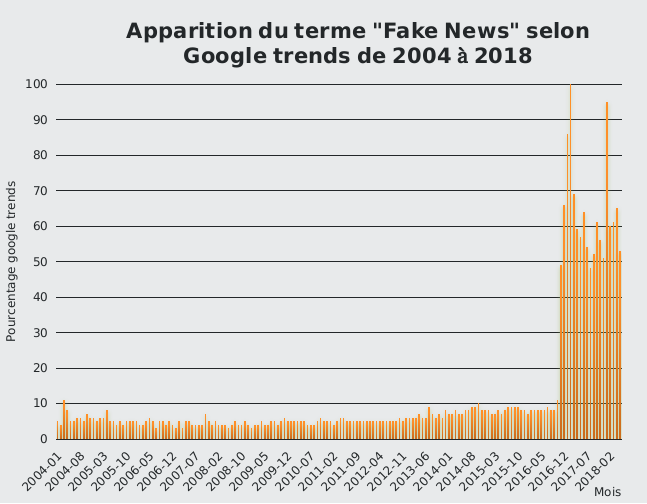
\includegraphics[scale=0.7]{../../img/google_trends.png}
 \captionof{figure}{Évolution de l'intérêt pour la recherche «\textit{Fake News}»}
 \footnote{L'Évolution de l'intérêt pour une recherche est ainsi définit par google:
  Les résultats reflètent la proportion de recherches portant sur un mot clé donné dans une région et pour une période spécifiques, par rapport à la région où le taux d'utilisation de ce mot clé est le plus élevé (valeur de 100). Ainsi, une valeur de 50 signifie que le mot clé a été utilisé moitié moins souvent dans la région concernée, et une valeur de 0 signifie que les données pour ce mot clé sont insuffisantes.}
 \label{google_trends}
\end{center}


\subsection{Le système monétaire des \textit{Fake News}.}


%Explication rapide du clickbait.
Le clickbait désigne un contenu web qui vise à attirer le maximum de passages d'internautes afin de générer des revenus publicitaires en ligne.
Le clickbait affiche des gros titres racoleurs.
Il est souvent mensonger et sensationnel.
L'exactitude et les sources de l'article sont inexistantes.
Le but du clikbait est d'être partagé massivement sur les réseaux sociaux.

%Comment le clickbait est utilisé dans la presse actuelle ?
Maintenant que la presse virtuelle est multiple, pour être rentable, elle doit générer une offre publicitaire non négligeable.
Le clickbait est un effet pervers d'internet.
Les possesseurs de contenu peuvent gagner de l'argent par le biais de la publicité.
Cela crée des nouveaux systèmes monétaires.

La ville de Vélès en Macédoine est devenue  le temps des élèctions américaines une \href{https://fr.sputniknews.com/international/201709251033204687-macedoine-veles-fake-news-trump/}{«[...] usine à \textit{Fake News} [...]».} En tous cas c'est ce que titre le sputniknews, en effet sur ces pages il propose l'interview de Dimitr, étudiant en Web-design qui cherchait à ce faire de l'argent facilement. «A un moment donné [Dimitr] et les [autres] étudiants ont compris qu'il était possible de gagner de l'argent avec la publicité en écrivant des nouvelles selon une équation simple: plus il y a de lecteurs, plus cela rapporte de l'argent.[...] La plupart d'entre eux publiaient des articles pour soutenir Trump, ou sur lui.»

%Les \textit{Fake News} le premier client du clickbait.
Les \textit{Fake News} et le clickbait associés répondent à la crise profonde de la presse papier au profit des réseaux sociaux comme médias.
De plus les \textit{Fake News} alimentent une méfiance envers les médias traditionnels.
Elles font croire avec leurs « faits alternatifs» qu'on tente de cacher quelque chose à la population.
Ainsi ce nouveau type de média essaye de conserver au plus son lectorat pour conserver des rentrées d'argent constantes.

\subsection{Raisons idéologiques.}
%Instrumentalisation de l'information pour servir un propos politique.
Les raisons idéologiques de produire des \textit{Fake News} ne manquent pas.
En particulier en politique, où elles sont utilisées à tout va.
%Exemple Pizzagate Hillary Clinton
Un exemple probant est le Pizzagate.
En résumé le Pizzagate est une « théorie» conspirationniste prétendant qu'il existe un réseau de pédophilie autour de John Podesta, l'ancien directeur de campagne d'Hillary Clinton.
Cette histoire fut rapidement démentie par les services de police et une majorité des médias américains. Mais les conséquences ne sont pas négligeables.
Un fusillade, heureusement sans blessé, a eu lieu dans la pizzeria où étaient soi-disant séquestrés les enfants du réseau pédophile de Podesta.


\section{Les origines des \textit{Fake News}.}

\subsection{Des médias négligents.}
La négligence et l'unicité des médias fait que les \textit{Fake News} peuvent se propager facilement.
Comme nous l'avons dit précédemment, les médias traditionnels traversent une crise.
La production de contenus doit être faites le plus rapidement possible.
Dans le but de répondre à la course à l'information de plus en plus grande et déloyale, la qualité des articles est revue à la baisse.
Certains journalistes ne font pas le travail de vérifier leurs sources pour accélérer le procédé de publication.



\subsection{Des organisations malveillantes internationales.}
L'appât du gain facile que sont les \textit{Fake News} a suscité des vocations.
Comme nous l'avons dit précédemment, une partie de la jeunesse de Vélès s'est ainsi spécialisée dans la création de \textit{Fake News}, attirée par de juteux revenus publicitaires. La ville s'est transformée en fabrique à \textit{Fake News} pendant l'élection américaine\footnote{Un autre article en parlant du \href{http://www.lefigaro.fr/actualite-france/2017/03/06/01016-20170306ARTFIG00187-fake-news-un-meme-terme-pour-plusieurs-realites.php}{Figaro} 20/12/2017 }.
Mais aussi des sites comme \href{https://www.infowars.com/}{InfoWars} voient naître des \textit{Fake News}.

\begin{center}
 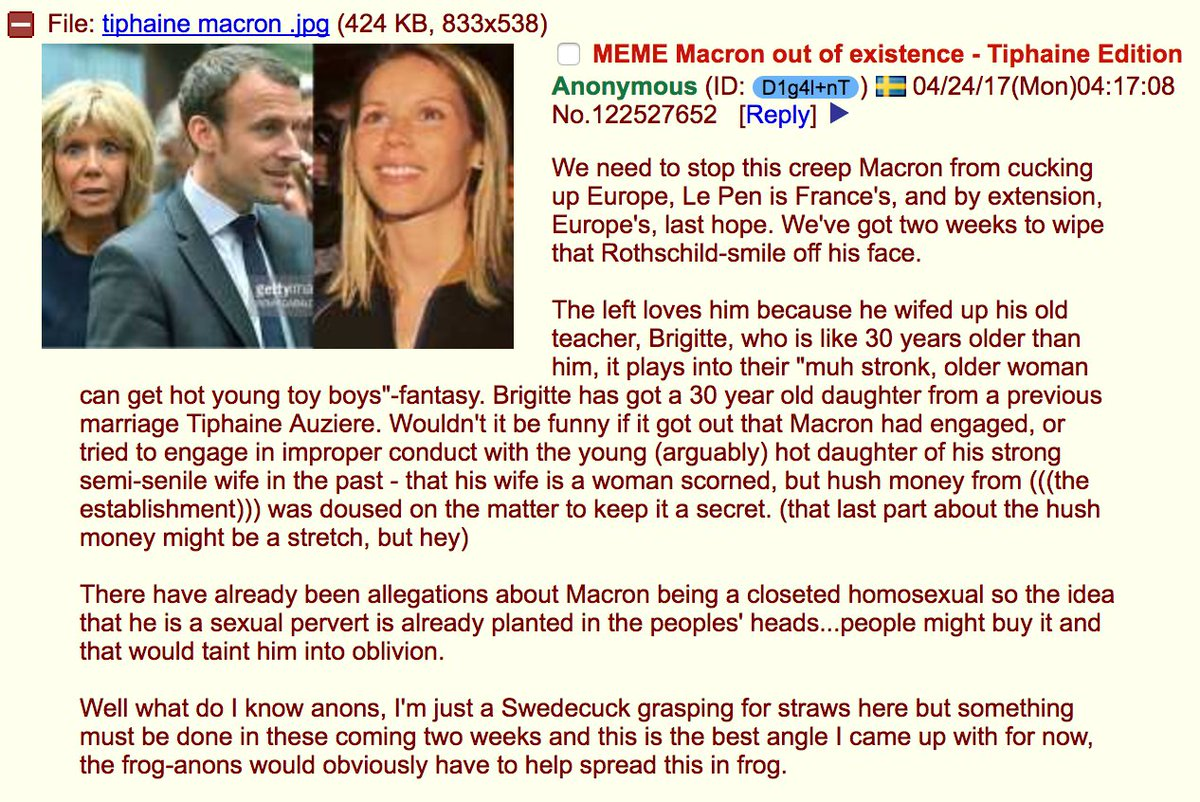
\includegraphics[scale=0.20]{../../img/rumeur_4chan/macron.jpg}
 \captionof{figure}{Capture d'écran d'un fil de discussion sur 4chan pour lancer une rumeur de pédophilie sur Macron.}
 \label{macron}
\end{center}

Des organisations qui travaillent dans l'ombre des plus grands forums sont à la base de la conception des \textit{Fake News}.
En effet, l'étude de \href{https://arxiv.org/abs/1705.06947}{Savvas Zannettou et al, 2017} montre comment les forums leaders mondiaux que sont 4chan et reddit sont en partie responsable dans la création de rumeurs.


\section{La propagation des \textit{Fake News}.}


\subsection{Les réseaux sociaux : médiations des \textit{Fake News}}
Selon \href{https://hal.inria.fr/hal-01281190}{Maksym Gabielkov et al, 2016}, 59\% des liens partagés sur Twitter n'ont jamais été cliqués.
En d'autres termes, la plupart des gens semblent retweeter des nouvelles sans jamais les lire.
Les personnes qui partagent sans lire des articles propagent certainement des \textit{Fake News} sans le savoir.

Pour évaluer une \textit{Fake News} nous n'avons pas besoin de dîplome.
En effet les déterminismes sociaux ne sont pas suffisants pour prévoir le partage de \textit{Fake News}.
L'éducation, le sexe, l'âge, etc. ne sont pas des critères distinctifs.
Nous pouvons inférer cela de l'étude \href{https://jean-jaures.org/nos-productions/le-conspirationnisme-dans-l-opinion-publique-francaise}{«Le conspirationnisme dans l’opinion publique française»}. Dans cette étude, on affirme qu'un français sur quatre sans distinction de sexe ou d'age croyait à au moins une théorie du complot. L'échantillon de 1250 personnes est représentatif de la population francaise. Si intrasequement les personnes croit à des théories qui ne sont pas la vérité, il est peu étonnant que les \textit{Fake News} soient autant partager sur les réseaux sociaux.

Ou pourait se demander
\href{http://esj-pro.fr/pourquoi-tout-le-monde%E2%80%8A-%E2%80%8Aou-presque%E2%80%8A-%E2%80%8Apartage-des-fake-news/}{
 «Pourquoi tout le monde - ou presque - partage des \textit{Fake News} ?»} La réponses se trouve en partie dans le
\href{http://www.digitalnewsreport.org/}{«Digitial News Report 2017»}
ou il est décrit que «51\% des adultes Américains s’informent sur les réseaux sociaux, contre 38\% en France».

Nous voyons alors que personne est à l'abri des \textit{Fake News}. Seuls la pensée critique et le recul nous permettraient d'être protégés des \textit{Fake News}.


\subsection{Le biais de confirmation.}
Les biais de confirmation sont un aspect déroutant de la pensée humaine.
Nous pourrions penser que l'homme ait acquis une pensée analytique développée pour arriver à ce niveau d'intelligence.
Et pourtant il est soumis au biais de confirmation.
Ce biais cognitif consiste à privilégier les informations confirmant nos idées préconçues ou nos hypothèses.
De plus il nous fait aussi négliger les informations jouant en défaveur de nos conceptions.

Ainsi les personnes tenantes de la thèse « des extraterrestres gouvernent le pays» sont plus enclin à croire la thèse « des reptiliens au pouvoir » que la thèse « Barack Obama est un être humain ».

Les \textit{Fake News} relayant souvent des informations conspirationnistes, il est facile pour un tenant de croire celle-ci plutôt que de croire des versions officielles.
Le biais de confirmation agit dans tous les sujets confondus.
Il n'est pas uniquement cantonné au conspirationnisme.
Les \textit{Fake News} utilisent ce biais de manière idéologique pour renforcer nos croyances et nous rendre son information plausible.

\href{http://www.rtl.fr/actu/debats-societe/des-anti-immigration-prennent-des-sieges-de-bus-pour-des-femmes-voilees-7789583989}{«Des anti-immigration prennent des sièges de bus pour des femmes voilées»}.
Sinder Beyer, un politicien norvégien, dénonce l'utilisation abusive d'une photo de siège de bus et l'idéologies raciste que prônent les anti-immigration sur un de leur poste facebook. Nous avons bien ici un renforcement des croyances prennant ces bases dans un \textit{Fake News}. C'est parce que ce groupe anti-immigration pense que la Norvège est envahie petit à petit par des musulmans qu'ils confondent des sièges d'autobus avec des femmes en burka.

\begin{center}
 
\includegraphics[scale=0.50]{../../img/femmes_musulmanes.png}
 \captionof{figure}{Poste de Sindre Beyer pour dénoncer l'erreur des anti-immigration.}
 \label{femmes_musulmanes}
\end{center}



\subsection{Tri de l'information selon Kahneman.}
La thèse centrale de Daniel Kahneman, dans son livre « Système 1 / Système 2 : Les deux vitesses », est qu'il y a une dichotomie entre deux modes de pensée.
Le système 1 est rapide, instinctif et émotionnel, alors que le système 2 est plus lent, plus réfléchi et plus logique.
Il définit les biais cognitifs associés à chacun de ces modes de pensée.
Il montre que l'on donne une trop grande importance au jugement humain.

Selon Kahneman nous nous reposons plus souvent sur le système 1.
Ce qui expliquerait notre partage de \textit{Fake News} quand nous sommes émotionnellement impliqués.

Imaginons qu'une personne antivax «ouverte d'esprit» voit cette article apparaître sur son fil d'actualité facebook, et qu'on lui demande d'évaluer la fiabilité de cette information:
\href{https://healingoracle.ch/2018/02/20/now-its-official-fda-announced-that-vaccines-are-causing-autism/}{\textit{«NOW IT’S OFFICIAL: FDA Announced That Vaccines Are Causing Autism!»}}. Cette personne devant traiter l'inforamtion rapidement va utiliser un argument d'autorité de sa communauté pour nous répondre que cette information est vrai. Elle a utilisé un raisonnement intuitif (système 1).
Maintenant on lui dit demande croiser les informations, remonter les sources et d'évaluer sérieusement les preuves avec des calcules comparatifs avec des expériences témoins. Si cette personne fait bien sont travail elle devait tomber sur un article du genre \href{http://www.politifact.com/punditfact/statements/2017/dec/19/truthcommandcom/no-fda-didnt-hide-information-linking-vaccine-auti/}{\textit{«No, the FDA didn't hide information linking vaccine to autism»}}. Et trouver peut des différences statistiquement non-significatives dans le pourcentage d'autiste chez les enfants vaccinés par rapport aux enfants non-vaccinés. Ici elle aura eu un raisonnement analytique et scientifique, mais qui lui aura pris beaucoup de temps (système 2).
Et si cette personne est vraiment ouverte d'esprit et de bonne foi, elle devrait changer un peu ses opinions sur les vaccins. Car elle aura eu les preuves tangibles sous les yeux. Ce ne veut pas dire qu'elle doit totalement changer d'avis mais qu'elle devra considérer que moins nocifs les vaccins. Ou du moins qu'ils ne causent pas l'autisme.


\section{Les risques des \textit{Fake News}.}

\subsection{Les risques politiques.}
%Comment les \textit{Fake News} peuvent aider à cacher des scandales politiques.
L'institutionnalisation des \textit{Fake News} est l'un des plus gros risques politiques.
En effet rien de pire qu'une \textit{Fake News} qui a pour pseudo-autorité un état.
Un état niant les faits devient répressifs.
%Exemple les alternatives facts de l'institution de Donald Trump.
\begin{center}
 \begin{figure}[h]
  \begin{subfigure}{.5\textwidth}
   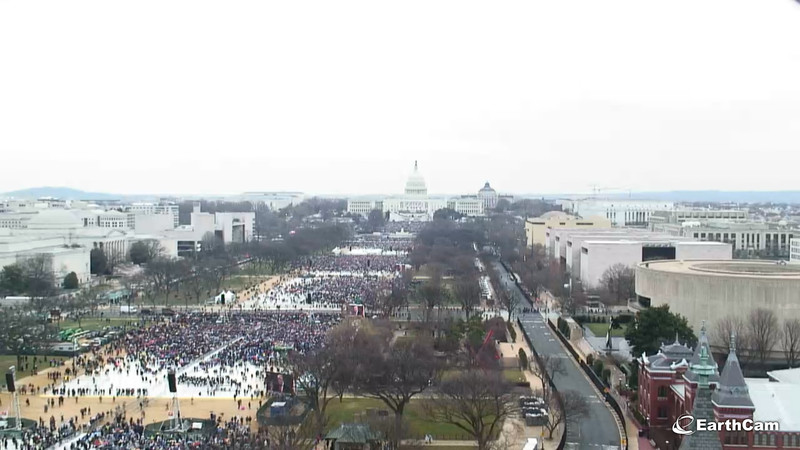
\includegraphics[scale=0.240]{../../img/trumpvswomen/trump.png}
   \caption{L'inauguration de Trump}
   \label{fig:sub1}
  \end{subfigure}
  \begin{subfigure}{.5\textwidth}
   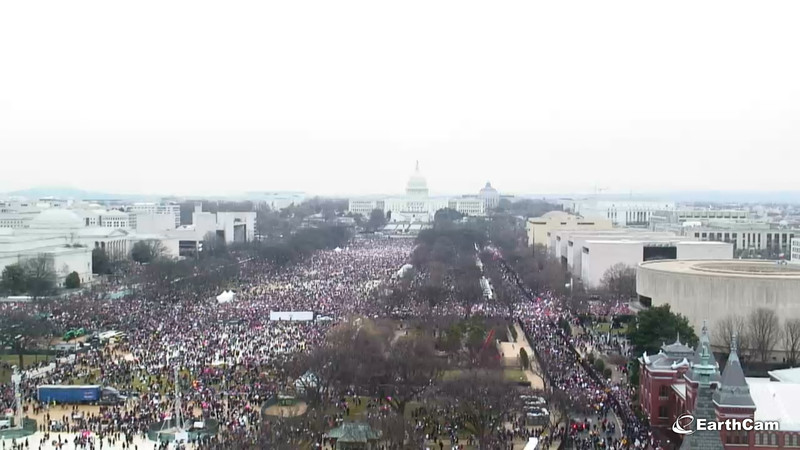
\includegraphics[scale=0.240]{../../img/trumpvswomen/women.png}
   \caption{Women’s March}
   \label{fig:sub2}
  \end{subfigure}
  \caption{Deux photos d'événements du National Mall à Washington}
  \label{fig:test}
 \end{figure}
\end{center}

L'inauguration de Trump et la Women's March avaient fait beaucoup de bruit.
Les partisans pro-Trump seraient soi-disant en plus grand nombre que les partisans de la Women's March.
Nous pourrions croire la version officielle.
Mais apparemment sans comptage, il y avait plus de participants à la Women's March.
L'État américain avaient tenté de faire passer cela pour des faits alternatifs.
Ce qui n'a pas beaucoup de sens.
Certes, nous observons tous le réel de manière différente, mais ce n'est pas une raison pour faire du relativisme et conclure à des faits alternatifs.
De plus comment définir des faits alternatifs ?
Prendre des faits et les dénaturer à des fins idéologiques ne nous donne pas raison sur la réalité.
En somme, les \textit{Fake News} peuvent servir à cacher des scandales politiques.

D'autres \textit{Fake News} institutionnalisées peuvent servir à des particuliers pour qu'ils puissent s'enrichir, ou à ne pas payer d'amende.
Par exemple, nier le réchauffement climatique est très pratique quand on est l'un des pays les plus polluant au monde.

\begin{center}
 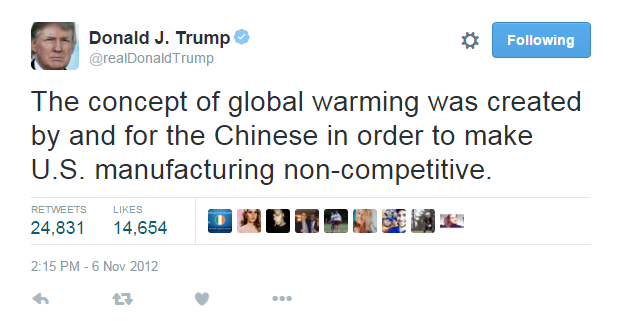
\includegraphics[scale=0.50]{../../img/globalwarming.png}
 \captionof{figure}{\href{http://www.politifact.com/truth-o-meter/statements/2016/jun/03/hillary-clinton/yes-donald-trump-did-call-climate-change-chinese-h/}{Tweet de Donald trump niant le réchauffement climatique.}}
 \label{globalwarming_trump}
\end{center}

\href{https://www.lexpress.fr/actualite/monde/amerique-nord/donald-trump-sort-les-etats-unis-de-l-accord-de-paris-sur-le-climat_1914113.html}{«Donald Trump sort les États-Unis de l'Accord de Paris sur le climat »}.
Comme promis dans sa campagne Donald Trump ne souhaite pas toucher aux emplois américains.
Il ne va pas prendre des mesures écologiques en ce qui concerne l'industrie des États-Unis.
Ainsi il décide de ne pas se joindre aux efforts des différentes nations pour diminuer la température global de deux degrès celcius.

\subsection{Les risques sanitaires.}
%Comment la santé peut être mise en danger par de fausse informations?
Beaucoup de \textit{Fake News} portent sur les domaines sanitaires.
Comme nous l'avons vu précédemment avec les vaccins, les \textit{Fake News} développent une méfiance pour la médecine conventionnelle.
Pour reprendre l'exemple des vaccins, il faut savoir que des cas de rougeole mortels sont réapparus ces dernières années.
Par exemple:
\href{https://www.tdg.ch/suisse/Les-cas-de-rougeole-ont-double-en-une-annee/story/25575100}{«Les cas de rougeole ont doublé en une année»} ou bien encore \href{https://www.la-croix.com/Sciences-et-ethique/Sante/rougeole-continue-etre-mortelle-France-2018-02-13-1200913536}{«La rougeole continue à être mortelle en France»}
Ne pas se vacciner entraîne un baisse de la couverture vaccinale.
Le rapport bénéfice/risque est plus que positif pour la vaccination.
Aucun des effets indésirables notoires suspectés n'a trouvé un protocole testable positif.
Nous n'avons que des affirmations pseudo-scientifiques et des hypothèses contre.
En somme, la désinformation, autour de la médecine notamment, peut couter la vie.



\subsection{Détournement des news vers des sujets clivants.}
Comme nous avons pu le voir précédement les \textit{Fake News} peuvent être colportées par des personnes convaincues de leur véracité.
Le but ultime d'une \textit{Fake News} est d'être considéré comme une vraie information.
Les \textit{Fake News} détournent l'attention de la population vers des problèmes factices et souvent résolus depuis des années. En somme les \textit{Fake News} sont une perte de temps. Elles nous empêchent de nous focaliser sur de vrais problèmes ; car l'on doit démystifier des faits irréels.



\section{Légitimité du projet et motivations.}

Comme nous avons pu le voir dans les sous-sections précédentes.
Les \textit{Fake News} sont de fausses nouvelles qui cherchent à tromper volontairement.
Elles participent pour la majorité à une pollution du web dûe au système monétaire de la publicité en ligne.
Elles servent parfois un propos idéologique avec de mauvais argument.
Ceci les rend moins crédibles pour ceux qui découvrent le pot aux roses.
Elles sont produites par des militants anonymes anti-intellectuels prônant la désinformation sur de sombres forums.
Elles inondent les réseaux sociaux d'inepties et sont partagées en masse sans être lues.
Elles véhiculent des titres avec de fausses idées alors qu'un simple coup d'oeil au corps de l'article rend le propos infondé.
De plus,Elles coutent la vie à certains.
Et pour finir elles peuvent devenir un instrument politique redoutable et autoritaire.

Pour toutes ces raisons il est légitime de vouloir combattre le phénomène des \textit{Fake News}.


\section{Comment détecter une \textit{Fake News}?}


\subsection{Comment vérifier des informations ?}
%Exposer différentes méthodes pour les différents types de médias.
Il y a deux moyens de détecter une \textit{Fake News}.
Par soi-même en cherchant les indices du canular.
Ou en utilisant un moteur de recherche de canular sur un domaine internet.

Premièrement voyons de manière non-exhaustive quelques techniques pour détecter une \textit{Fake News}:
\begin{description}
 \item [Avant de partager] il faut se questionner sur ce qu'il est raconté dans l'article et vérifier les sources. On est responsable de ce que l'on partage.
 \item [Est-ce une information ?] Il faut se poser différentes questions: Est-ce cela à un intérêt public ? Est-ce factuel ? Est-ce vérifié ? Cela permet de distinguer les avis et les rumeurs des informations.
 \item [Ce site est-il fiable ?] A-t-il une page « À propos » ? Est-il parodique ? Quelles sont les sources de ce site ?
\end{description}
Beaucoup de techniques spécifiques pour chaque média existent ! Nous ne pouvons pas être exhaustif ici.

Les \textit{Fake News} ont fait apparaître de nouveaux sites spécialisés dans la détection de canulars.
Par exemple, en français, il existe le \href{http://www.lemonde.fr/verification/}{Décodex} propulsé par le journal le Monde. Ce site répertorie les autres sites selon leurs fiabilités.
En anglais il existe le site internet Polifacts de vérification des faits, qui vérifie la véracité des promesses et engagements pris par les politiques américains
%\paragraph{Les limites des MDR vérificateur de faits.}
%Premièrement passer des menottes au lieu d'ouvrir le débat n'est pas une bonne solution !

%Deuxièmement les conflits d'intérêts des grands groupes qui font du fact-checking n'est pas à négliger. Une source de connaissance univoque n'est pas objective.
\subsection{Méthode informatique actuelle: \textit{Stance Detection}.}
Cette tâche peut aussi être résolue avec un succès modeste par l'apprentissage automatique.
En effet une des réponses au phénomène des \textit{Fake News} est l'apparition de réseaux neuronaux complexes qui permettent de manière partielle de repérer les \textit{Fake News}. Ce repérage passe par une détection des partis pris (stance detection).

Ainsi dans la deuxième partie de ce mémoire, nous allons voir plus en détail ce qu'est la stance detection.
Au travers de tâches partagées, nous allons découvrir les techniques pour l'utiliser.

Dans la troisième partie nous nous essayerons à la Stance detection aussi.
Et donnerons une analyse comparative de nos résultats par rapport à l'état de l'art.


\chapter{État de l'art: \textit{Stance Detection}}

\begin{abstract}
 Dans cette partie nous allons présenter la \textit{Stance Detection} et lui donner une définition rigoureuse.
 Nous discuterons les différentes tâches partagées qui ont eu lieu autour de la \textit{Stance Detection}. Notamment nous présenterons les corpus et les méthodes de classification choisies.
\end{abstract}

\section{Vers une définition.}
\subsection{Formalisation de la \textit{Stance Detection}.}
La \textit{Stance Detection} ou en français la détection de parti pris
\footnote{Vous remarquerez que pour la cohérence et pour la consistance de ce document nous  n'emploierons plus que la formulation « détection de parti pris» au lieu de «\textit{Stance Detection}».}
est la méthode qui permet de déterminer si un énoncé \textbf{E} par rapport à une cible \textbf{C} donnée est en accord ou en désaccord avec la cible.
On l'utilise aussi parfois pour déterminer si l'énoncé discute sans parti pris de la cible.
C'est-à-dire que \textbf{E} parle de \textbf{C} mais on ne trouve aucun indice soit en faveur, soit en défaveur la cible.
Par extension, si on arrive à déterminer la cible, on peut connaître les énoncés qui n'y correspondent pas.
Ce type d'énoncé indépendant ne donne aucun indice de prise de parti et surtout aucun indice de la cible en général.
La cible et l'énoncé ne partagent aucun lien direct ou indirect.
Ainsi la détection de parti pris nous permet de repérer ces quatre cas de figure:

\begin{description}
 \item [E est pour C] quand l'énoncé montre un ou des indices en faveur de la cible.
 \item [E est contre C] quand l'énoncé montre un ou des indices en contradiction avec la cible.
 \item [E discute C] quand l'énoncé donne une ou des informations sur la cible sans donner d'indices de parti pris comme dans les deux cas pécédents.
 \item [E est non-lié à C] quand l'énoncé ne donne aucune information par rapport à la cible en général.
\end{description}

Les deux derniers cas ne détectent aucun parti pris.
Mais ils restent pertinents pour la détection de parti pris doit intégrer une limitation à un sujet donné.
Une telle détection implémente donc un module de détection des relations.
Appellons \textbf{R} la relation entre \textbf{E} et \textbf{C}.


\subsection{Domaine de la détection de parti.}
Nous avons beaucoup parlé d'indices dans la partie précédente.
Questionnons leur nature.
La détection de parti pris se base sur la relation entre la cible et l'énoncé.
La nature de cette relation est sémantique.
Les traits qui permettent d'unir l'énoncé et la cible pour déterminer le parti pris doivent alors aussi entretenir une relation sémantique.
On verra plus tard que certaines relations syntaxiques peuvent être utiles de manière localisées dans certaines tâches.

Il apparait un problème dû à la sémantique: il faut s'accorder au préalable sur le sens des mots et sur ce que désignent nos cibles et leurs rapports avec l'énoncé.
En effet, pour constituer un corpus de prise de position par rapport à un énoncé, il faudra trouver la manière la plus objective de qualifier la relation entre l'énoncé et la cible.
\subsection{La genèse de la détection de parti pris.}

Une des premières publications sur la déctection de prise de parti était «  \textit{Cats Rule and Dogs Drool![...]} » (voir \href{http://www.aclweb.org/anthology/W11-1701}{Pranav Anand et al, 2011}) qui cherchait à classer la prise de position dans des débats en ligne sur des sujets variés.
Leur but était de montrer que les débats idéologiques comportent une plus grande part de messages de réfutation.
La publication montrait aussi qu'il est beaucoup plus difficile de classer les posts de réfutation, aussi bien pour les humains que pour les classificateurs automatiques formés à la détection de prise de parti.

Les chercheurs ont créé leur corpus à partir de 1113 débats bi-partiaux (soit 4873 posts) dans 14 sujets différents du site \href{http://www.convinceme.net/}{ConvinceMe.net}.
Pour annoter le corpus, les chercheurs ont demandé à neuf participants de mettre une étiquette sur différentes parties de débat sur le site.
Il est intéressant de notifier que les annotateurs  n'ont eu que 0.73 d'exactitude croisée dans la classification des réfutations (tous sujets confondus).
Ainsi le problème sémantique est réel.
Les annotateurs ne tombent pas d'accord sur la relation sémantique de certains énoncés par rapport à leurs cibles.
Le but d'un système automatique de classification des réfutations sera donc de s'approcher au plus de ce pourcentage d'exactitude pour représenter au mieux le classement humain général.

L'équipe d'Anand a fait plusieurs modèles de système utilisant des traits différents (n-grams, la ponctuation répétée, LIWC, dépendance syntaxique,...).
Ces modèles utilisaient soit une implémentation de Naive Bayes, soit une implémentation de JRip\footnote{JRip est un classificateur basé sur des règles qui produisent un modèle compact adapté à la conception d'application rapide.} en fonction des traits choisis.

Les résultats des modèles varient en fonction des sujets entre 0.59 et 0.69 d'exactitude pour la détection de réfutation.
De plus, aucun modèle ne se départage des autres.
Tous ont plus ou moins réussi selon un sujet différent.
La moyenne est 0.63 pour la détection de réfutation.
C'est dix points de moins que l'exactitude humaine (qui varie entre 0.66 et 0.94).

Premièrement, cette publication nous montre combien il est ardu de se confronter à la sémantique.
En droit, le sens d'un énoncé devrait être univoque et susciter une seule relation universelle entre la cible et l'énoncé.
En fait, nous -les annotateurs humains- sommes tous soumis à des biais, des opinions, des préjugés qui ne permettent qu'un recouvrement subjectif de la relation entre cible et énoncé.

Deuxièmement, ce papier montre la difficulté de la tâche.
Aucun modèle possédant des traits particuliers n'a eu de meilleur résultat dans tous les sujets confondus.

Nous avons présenté un des premiers travaux sur la détection de parti pris.
Par la suite, nous nous limiterons à des travaux plus récents.
Ceux-ci s'intéressent à notre sujet: les \textit{Fake News}.

\subsection{Application générale et relative au \textit{Fake News}.}
Nous allons voir dans les sections suivantes les différentes utilisations de la détection de parti pris à travers deux tâches partagées.
Premièrement dans la section \no2, nous verrons l'utilisation de la détection de parti pris à l'intérieur de \textit{tweets} sur des sujets polémiques; grâce à la \textbf{\textit{SemEval-2016 Task 6}}.
Puis deuxièmement dans la section \no3, nous verrons l'utilisation de la détection de parti pris pour la détection de \textit{Fake News} ; grâce au \textbf{\textit{Fake News Challenge}}.
Nous proposerons dans la troisième partie de ce mémoire une contribution originale de la tâche que nous discutons dans la section \no3.



%%%%%%%%%%%%%%%%%%%%%%%%%%%%%%%%%%%%%%%%%%%%%%%%%%%%%%%%%%%%%%%%%%%%%%%%%%%%%%%
%%%%%%%%%%%%%SemEval-2016 Task 6%%%%%%%%%%%%%%%%%%%%%%%%%%%%%%%%%%%%%%%%%%%
%%%%%%%%%%%%%%%%%%%%%%%%%%%%%%%%%%%%%%%%%%%%%%%%%%%%%%%%%%%%%%%%%%%%%%%%%%%%

\section{\textit{SemEval-2016 Task 6}.}
\subsection{Description générale de la tâche.}
Cette tâche porte le nom de « \textit{Detecting Stance in Tweets} » (\href{https://www.aclweb.org/anthology/S/S16/S16-1003.pdf}{Saif M.
 Mohammad et al, 2016}).
Le but de la tâche est de déterminer la relation \textbf{R} entre un tweet \textbf{E} et une cible \textbf{C}.

Ici, nous avons trois classes possibles pour déterminer le parti du tweeter par rapport à son tweet:
\begin{description}
 \item [favor] s'il est en faveur la cible.
 \item [against] s'il est contre la cible
 \item [neither] si il n'est ni en faveur la cible, ni il n'est contre la cible.
\end{description}

Exemple direct:

\begin{description}
 \item [C] Hillary Clinton
 \item [E] Hillary Clinton has some strengths and some weaknesses.
 \item [R] neither
\end{description}

Exemple indirect:
\begin{description}
 \item [C] legalization of abortion
 \item [E] A foetus has rights too! Make your voice heard.
 \item [R] against
\end{description}

\newpage
La tâche se divise en deux sous-tâches:
% la première \textbf{A} supervisée et la deuxième \textbf{B} non-supervisée.

\subsubsection{Sous-tâche A.}
La sous-tache A est supervisée.
Elle porte sur cinq différents sujets (\textit{‘Atheism’},\textit{ ‘Climate Change is a Real Concern’},\textit{‘Feminist Movement’}, \textit{‘Hillary Clinton’},\textit{‘Legalization of Abortion’}).
Elle contient 4163 couples \textbf{C/E} labélisés \textbf{R}.
On réserve 30\% pour l'ensemble de test et le reste pour l'ensemble d'entraînement.

\subsubsection{Sous-tâche B.}
La sous-tache B est non-supervisée.
Elle porte sur un seul thème (\textit{‘Donald Trump’}).
L'ensemble test est constitué de 707 tweets \textbf{E}.
Aucun ensemble d'entraînement n'a été donné.
Mais un ensemble de 78 000 tweets non-labélisés à propos de Donald Trump était disponible.

\subsubsection{Évaluation.}
Pour l'évaluation des systèmes on utilise le F1-score moyen; calculé ainsi:
\begin{equation}
 F_{avg} = \frac{F_{favor}+F_{against}}{2}
\end{equation}

\subsection{Les participants.}
Il y a eu 19 dépots pour la sous-tâche A et 9 dépots pour la sous-tâche B.
Premièrement, nous parlerons de la réussite à la tâche en général.
Deuxièment, nous discuterons seulement de quelques dépots intéressantes.
Et troisièment, nous comparerons les différents protocoles vus.

\subsubsection{Dépots en général.}
Parmi les 19 dépots de la sous-tâche A aucun système n'a dépassé les baselines.
En effet, Saif M.
Mohammad et al ont fourni 4 baselines pour la sous-tâche A.
La première baseline naïve donnait le label majoritaire à toutes les entrées (\textit{Majority class}).
Les trois suivantes utilisent un ou plusieurs classificateurs linéaires (SVM) pour labéliser les entrées.
La deuxième utilisent 5 classificateurs SVM (un pour chaque différent sujet) sur les vecteurs d'unigrams de la combinaison de \textbf{C} et \textbf{E} (\textit{SVM-unigrams}).
De la même manière la troisième a aussi 5 SVM mais utilise comme dimensions de vecteur :
les 1-2-3-grams pour les mots et les 2-3-4-5-grams pour les caractères (\textit{SVM-ngrams}).
Et pour finir, la quatrième baseline utilise un seul SVM sur les mêmes dimensions de vecteur que la troisième baseline (\textit{SVM-ngrams-comb}).

En revanche, 7 des 9 équipes ont réussit à battre les baselines de la sous-tâche sur B.
Ces baselines reprennent certaines baselines de la sous-tâche A à savoir la première  \textit{Majority class} et la quatrième \textit{SVM-ngrams-comb}.

Pour la sous-tâche A, la plupart des équipes ont utilisé des fonctions de classification de texte standard tels que n-gram et vecteurs de mots, des lexiques de sentiments.
Certaines équipes ont interrogé Twitter sur des hashtags, pour marquer des prises de parti plus déterminantes.
Certaines ont entrainé leurs systèmes à partir de  vecteurs de Google Actualitée ou directement des corpus Twitter.

Et pour la sous-tâche B, certaines équipes ont très bien détecté les tweets en faveur
de Trump. Grâce aux tweets qui se trouvaient dans le corpus de Clinton en inversant leur valeur.

\subsubsection{Dépots particuliers.}
Ici, de manière succinte, nous allons décrire les différents modèles des meilleurs systèmes pour les différentes tâches.

\paragraph{MITRE 1er pour la tâche A.}

\begin{center}
 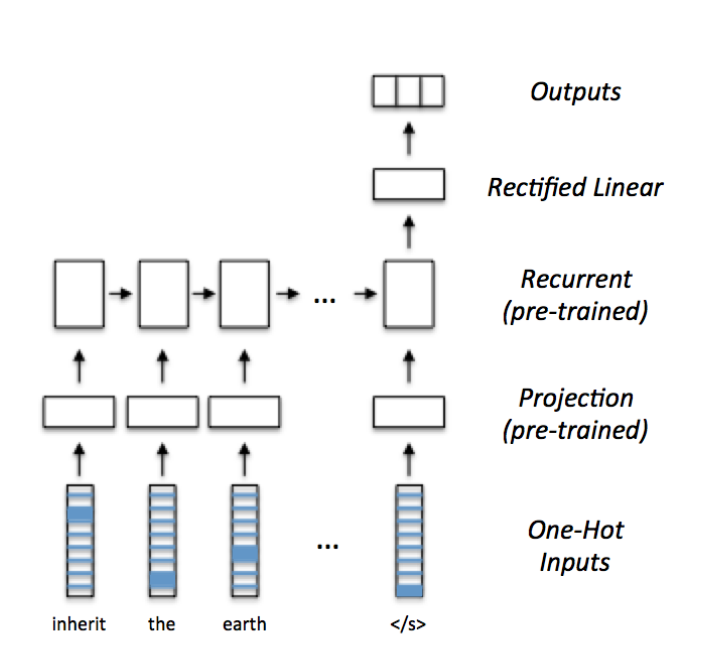
\includegraphics[scale=0.25]{../../img/model/mitre/model.png}
 \captionof{figure}{Le réseau neuronal récurrent de MITRE pour la détection de parti pris.}
 \label{mitre_model}
\end{center}

L'approche de détection de prise de parti de MITRE utilise un réseau de neurones récurrent organisé en quatre couches de poids.
Chaque mots est projeté comme une entrée dans une couche d'\textit{embbeding} de 256 dimensions (créé avec word2vec), qui alimente en une couche récurrente contenant 128 LSTM.
La sortie du terminal
de cette couche récurrente est densément connecté à un 128 classifieurs linéaires
Cette même couche est entièrement connectée à un softmax tri-dimentionnel dans laquelle chaque unité représente l'une des classes de sortie: FAVOR, AGAINST ou NONE.

\paragraph{pkudblab 2ème pour la tâche A.}
\begin{center}
 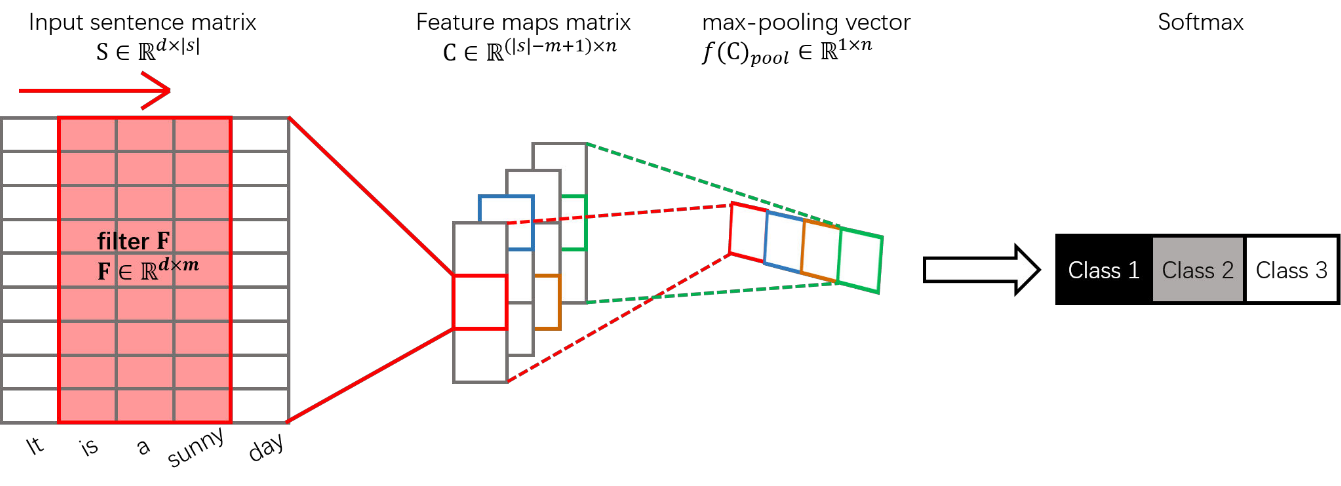
\includegraphics[scale=0.25]{../../img/model/pkudblab/model.png}
 \captionof{figure}{Architecture principale du réseau de neurones convolutionnels de pkudblab.}
 \label{pkudblab_model}
\end{center}
L'Architecture principale de pkudblab est un réseau de neurones convolutionnels.
On peut en décrire 5 composant majeurs:
\begin{description}
 \item[Une table de correspondance] est une énorme matrice d'embbeding de mots.
       Chaque colonne de la table, correspond à un mot.
       Chaque mot incorporé dans cette table a été pré-formé par des vecteurs de word2vec (Mikolov et al., 2013).
       Ces vecteurs sont formés sur une partie de l'ensemble de données Google News.
 \item[Une matrice d'entrée] représente d'une phrase d'entrée et la longueur de la phrase.
 \item[La couche convolution] a pour but d'extraire des paternes, de sorte que certaines formulations abstraites communnes soient représentées.
 \item[Le Pooling layer] a pour but est de simplifier l'information dans le
       sortie de la couche convolutionnelle.
 \item[La Couche de sortie softmax] est entièrement connectée et est destinée à la classification.
\end{description}

Pour la sous-tâche A, ils ont séparées les ensembles de données en cinq sous-ensembles.
Ils ont donc entrainé de manière séparé les modèles sur les différents sujets.

\paragraph{pkudblab 1er pour la tâche B.}

Pour la sous-tâche B, ils ont utilisé le même modèle que pour A.
Pour entraîner leur modèle ils établissent un ensemble de données de formation à deux classes (favor, against) à partir du corpus du domaine officiel en fonction de plusieurs expressions spéciales.

\subsubsection{Discussions comparatives.}
% tableau rérésultats tâches A
\begin{center}
 \begin{tabular}{| c | c | c || c |}
  \hline
  \textbf{Baseline} & \textbf{F$_{favor}$} & \textbf{F$_{against}$} & \textbf{F$_{avg}$} \\
  \hline
  Majority class    & 52.01                & 78.44                  & 65.22              \\
  SVM-unigrams      & 54.49                & 72.13                  & 63.31              \\
  SVM-ngrams        & 62.98                & 74.98                  & 68.98              \\
  SVM-ngrams-comb   & 54.11                & 70.01                  & 62.06              \\
  \hline
  \textbf{Équipe}   &                      &                        &                    \\
  \hline
  MITRE             & 59.32                & 76.33                  & 67.82              \\
  pkudblab          & 61.98                & 72.67                  & 67.33              \\
  TakeLab           & 60.93                & 72.67                  & 66.83              \\
  \hline
 \end{tabular}
 \captionof{table}{Résultats pour la sous-tâche A des baselines et des 3 premiers participants ordonnés.}
\end{center}


% commentaires
On voit qu'il est difficile de faire décoller les scores mêmes avec les meilleurs systèmes.
Ceci nous donne une bonne idée de l'état de l'art en 2016.
Une implémentation simple avec des n-grams bien choisis et une catégorisation aident beaucoup à avoir de bons résultats.
Mais est-ce toujours possible de contextualiser les données ? Il y a un biais notoire du fait de  travailler avec une micro vocabulaire en plus souvent réduit sémantiquement par l'algorithme.
% tableau tâches B
\begin{center}
 \begin{tabular}{| c | c | c || c |}
  \hline
  \textbf{Baseline} & \textbf{F$_{favor}$} & \textbf{F$_{against}$} & \textbf{F$_{avg}$} \\
  \hline
  Majority class    & 0.00                 & 59.44                  & 29.72              \\
  SVM-ngrams-comb   & 18.42                & 38.45                  & 28.43              \\
  \hline
  \textbf{Équipe}   &                      &                        &                    \\
  \hline
  pkudblab          & 57.39                & 55.17                  & 56.28              \\
  LitisMind         & 30.04                & 59.28                  & 44.66              \\
  INF-UFRGS         & 32.56                & 52.09                  & 42.32              \\
  \hline
 \end{tabular}
 \captionof{table}{Résultats pour la sous-tâche B des baselines et 3 premiers participants ordonnés.}
\end{center}

La tâche dîte non-supervisée a fini par l'être.
Au final les équipes ont utilisé le corpus d'Hillary Clinton pour former celui de Trump.
Ils ont juste ajouté quelques expressions clichés trouvé la faveur ou la défaveur du tweet.
Le sujet de cette sous-tâche est particuliérement clivant.
Cela ne permet pas de retirer une méthode d'apprentissage non supervisé objective.

%%%%%%%%%%%%%%%%%%%%%%%%%%%%%%%%%%%%%%%%%%%%%%%%%%%%%%%%%%%%%%%%%%%%%%%%%%%%%%%%
%%%%%%%%%%%%%%%%FNC%%%%%%%%%%%%%%%%%%%%%%%%%%%%%%%%%%%%%%%%%%%%%%%%%%%%%%%%%%%%%
%%%%%%%%%%%%%%%%%%%%%%%%%%%%%%%%%%%%%%%%%%%%%%%%%%%%%%%%%%%%%%%%%%%%%%%%%%%%%%%%

\section{\textit{Fake News Challenge}.}

\subsection{Description générale de la tâche}
Nous présentons dans cette section la tâche partagée qu'est le \textit{Fake News Challenge} et les différentes solutions proposées par ses participants.
Pour détecter des \textit{Fake News} il nous faut résoudre plusieurs défis à savoir:
\begin{enumerate}
 \item Déterminer si les faits présents dans l'article de presse sont corrects; c'est-à-dire déterminer la véracité des faits par rapport au monde réel.
 \item Analyser les relations entre le titre de l'article et le corps de l'article.
 \item Quantifier le biais inhérent d'un texte.
\end{enumerate}
On voit clairement une application de la détection de parti pris dans le défi \no2.
En effet ce défi correspond parfaitement à sa définition.

Évaluer la véracité d'un article est une tâche complexe et lourde, même pour des experts formés.
La première étape du \textit{Fake News Challenge} se concentre sur la tâche de détection de parti pris.
\subsubsection{But.}
L'objectif du \textit{Fake News Challenge} est d'explorer comment les technologies
d'intelligence artificielle pourraient être utilisées pour lutter contre les
\textit{Fake News}.
\subsubsection{Organisation générale.}
Vous pouvez retouver toutes les infomations du \href{http://www.fakenewschallenge.org/}{\textit{Fake News Challenge}} sur leur site officiel.
Et vous pouvez retrouver les codes de leur \href{https://github.com/FakeNewsChallenge/fnc-1-baseline}{baseline} et \href{https://github.com/FakeNewsChallenge/fnc-1}{les données} sur github.


\subsubsection{Données et origines des données.}
Le FNC est une tâche partagée supervisée.
Les donneés sont pourvues par les organisateurs.
Ils définissent les données en termes d'entrées et de sorties.Une entrée est le couple formé par une affirmation \textbf{C} et un corps de texte \textbf{E}; soit à partir du même article de nouvelles ou de deux articles différents.
Une sortie est la relation \textbf{R} corps du texte par rapport à la revendication faite dans l'affirmation définie par l'une de ces quatre catégories:

\begin{description}
 \item [related:] Le corps du texte \textbf{E} et l'affirmation \textbf{C} traitent d'un sujet en commun\footnote{Cette méta-relation ne labélisera jamais les données elle est là pour mieux comprendre le but de la détection de prise de parti.}.
       \begin{description}
        \item [agree:] Le corps du texte \textbf{E} est en accord avec l'affirmation \textbf{C}.
        \item [disagree:] Le corps du texte \textbf{E} n'est pas d'accord avec l'affirmation \textbf{C}.
        \item [discuss:] Le corps du texte discute \textbf{E} le même sujet que l'affirmation \textbf{C}, mais ne prend pas de parti pris.
       \end{description}
 \item [unrelated:] Le corps du texte \textbf{E} traite d'un sujet différent de l'affirmation \textbf{C}.
\end{description}

\href{http://aclweb.org/anthology/N/N16/N16-1138.pdf}{Ferreira \& Vlachos (2016)} ont au préalable testé et créé un ensemble de donneés à partir du \href{http://www.emergent.info/}{site du projet Emergent} de Craig Silverman.
Le projet Emergent fut aussi utile pour la création du corpus de la FNC.

Les données de ce projet ont été collectées par des journalistes du \href{https://towcenter.org/}{\textit{Tow Center for Digital Journalism}}.
Pour ajouter une entrée au site, le journaliste doit trouver deux choses: une affirmation qui semble être une rumeur et un ensemble d'articles qui parlent de cette soi-disant rumeur.
Les sujets de chaque affirmation varient, cela va des dixits politiques de Donald Trump aux comparaisons de prix de la prochaine Apple Watch.
Les sources de celles-ci sont les comptes twitter polémiques, traitant les rumeurs et les sites tel que Snopes.com\footnote{\href{https://www.snopes.com/}{Snopes.com} est un site Web anglophone créé dans le but de limiter la propagation des canulars informatiques et des rumeurs infondées circulant sur Internet.}.À partir de certaines affirmations, le journaliste constitue donc un corpus d'articles pour établir la véracité de celles-ci.
Donc chaque affirmation peut être « Vraie», « Fausse» ou « Non-vérifié».
Cette valeur de vérité peut être établie grâce au corpus d'articles; où chaque article peut soit être « Pour», « Contre» ou « Neutre».
Le journaliste résume l'article en un gros titre (\textit{headline} à ne pas confondre avec notre affirmations de rumeurs).
Ce n'est pas le nombre d'articles « Pour»  ou « Contre» la véracité des affirmations; mais bien sur la vraissemblance des preuves qui sont rapportées dans les articles jugées par le journaliste.

Le corpus de Ferreira \& Vlachos est composé alors de 300 affirmations de rumeurs dont 2595 articles sont associés à un ratio de 8,75 articles pour une affirmation.
La distribution hétérogène  est de 47.7\% « Pour», 15.2\% « Contre» et 37.1\% « Neutre».
Pour tester si les données d'Emergent étaient assez discriminatives et robustes pour une tâche d'apprentissage automatique, Ferreira \& Vlachos ont testé l'accord entre les gros titre des journalistes et les affirmations de rumeurs.
Nous ne détaillerons pas plus leur protocole ici.
Mais leur 73\% d'exactitude (par rapport aux 47\% de leur baseline naïve) donne une bonne estimation de la consistance des données.

La répartitions des donneés de la FNC est faite avec le même procédé mais cette fois-ci on est extrait l'affirmation de rumeurs et le corps des articles.
De plus les organisateurs ajoutent une dimension de classification; la classe \textbf{unrelated}  est formée à partir des couples affirmation et de valeurs qui n'ont pas de liens sur la plateforme Emergent.
Les sujets sont alors non-liés.
La répartition des données au niveau des relations \textbf{R} se fait donc ainsi pour l'entrainement: 73.13\% sont \textbf{unrelated}, 17.82\% sont \textbf{discuss}, 7.36\% sont \textbf{agree} et 1.68\% sont \textbf{disagree}.
En chiffre cela donne 37727 corps d'articles \textbf{E} pour 1648 affirmations de rumeurs \textbf{C}.
Ce qui a donné 49973 couples \textbf{C/E}.
L'ensemble de test est composé de 20019 corps d'articles \textbf{E}, 894 affirmations de rumeurs \textbf{C} et donc de 25419 couples \textbf{C/E}.
Bien sûr, les données \textbf{E} ou \textbf{C} entre le test et l'entrainement ne se recoupent pas et les relations \textbf{R} ne sont pas données dans le test.

Voici un exemple de données pour l'affirmation \textbf{C} suivante « \textit{Robert Plant Ripped up \$800M Led Zeppelin Reunion Contract} »:

\begin{description}
 \item [R: Agree] \textbf{E}: « \textit{ … Led Zeppelin’s Robert Plant turned down £500 MILLION to reform supergroup.
        … } »
 \item [R: Disagree] \textbf{E}: « \textit{ … No, Robert Plant did not rip up an \$800 million deal to get Led Zeppelin back together.
        … } »
 \item [R: Discusses] \textbf{E}: « \textit{ … Robert Plant reportedly tore up an \$800 million Led Zeppelin reunion deal.
        … } »
 \item [R: Unrelated] \textbf{E}: « \textit{ … Richard Branson’s Virgin Galactic is set to launch SpaceShipTwo today.
        …} »
\end{description}



\subsubsection{L'évaluation.}
\begin{center}
 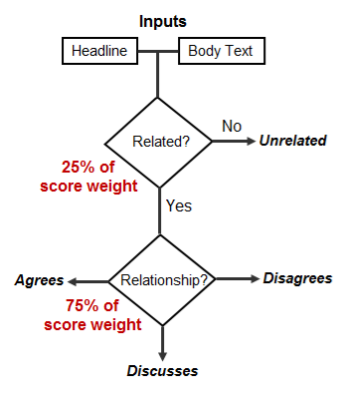
\includegraphics[scale=0.5]{../../img/fnc-eval/fnc-eval.png}
 \captionof{figure}{Diagramme de calcul du score relatif.
  Traduire ici « Headline» par \textbf{C} et  « Body Text» par \textbf{E}.}
 \label{fig_eval}
\end{center}

Les équipes seront évaluées selon un système de score relatif pondéré à deux niveaux; pour le premier niveau il faut classer \textbf{E} et \textbf{C} comme étant liés ou non (25\% de la pondération).
Puis pour le deuxième niveau il faut classer les couples liés comme étant d'accord, en désaccord ou discuté (75\% de la pondération), trouver le bon \textbf{R} du couple.
Le score relatif est le score brut normalisé par le score maximum possible sur l'ensemble de test \footnote{Nous donnerons à chaque fois le score brut et le score normalisé en pourcent.}.
En effet, il est très facile d'avoir une très bonne exactitude avec une classe sur-représentée comme les \textbf{unrelated} (73.13\% du corpus d'entrainement).
Il y a donc deux règles qui régissent ce score:
\begin{description}
 \item [unrelated/related :] si la classe Gold et la classe attiribué ont la même méta-classe alors on ajoute 0.25 au score.
 \item [same related :] si entre deux classe \textbf{related} la classe Gold et la classe attiribuée sont les mêmes, alors on ajoute 0.75 au score.
\end{description}

Exemples de scores en fonction de l'attribution de classe:

\begin{center}
 \begin{tabular}{| c | c || l | }
  \hline
  \textbf{Classe Gold} & \textbf{Classe attribuée} & \textbf{Score} \\
  \hline
  unrelated            & unrelated                 & +0.25          \\
  agree                & unrelated                 & +0             \\
  agree                & disagree                  & +0.25          \\
  agree                & agree                     & +0.75          \\
  \hline
 \end{tabular}
 \captionof{table}{Score en fonction de l'attribution de classe.}
\end{center}

\subsubsection{Baseline.}
Une simple baseline utilisant un classificateur de boosteur de gradient est fourni par les organisateurs.
Cette baseline inclut également le code pour le pré-traitement du texte, la division des données pour éviter des pertes entre l'entraînement et le test, la validation croisée avec k-fold.
Cette baseline permet les overlap entre les mots et les n-grams et des fonctions d'indicateurs pour la polarité et la réfutation.
Avec ces caractéristiques et un classificateur boosté, la baseline atteint un score d'exactitude pondérée de 79,53\% avec dix validations croisées.


\subsubsection{Les participants.}
Il y a eu 71 équipes participantes à cette tâche. Les trois premières équipes avaient pour obligations d'écrire un article sur leur système et d'en publier une version Opensource.
Dans les sous-sections qui suivent, nous allons justement vous présentez les systèmes des trois gagnant de FNC.

%########################################################################################
%##################Solat in the swen#####################################################
%########################################################################################


\subsection{Solat in the swen.}
\subsubsection{Méthodologie.}
\begin{center}
 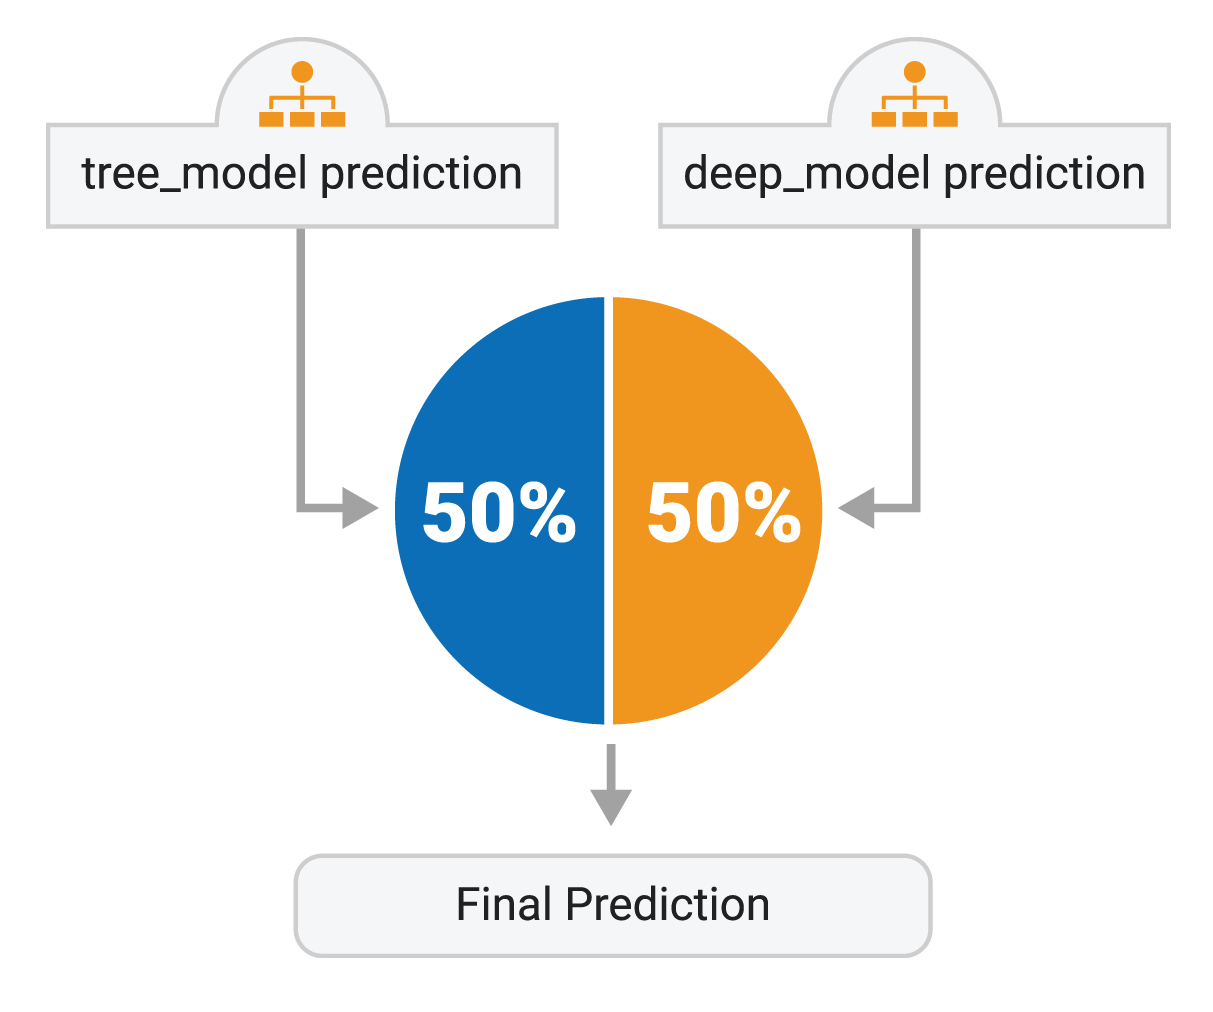
\includegraphics[scale=0.5]{../../img/model/solat_in_the_swen/final_prediction_light.png}
 \captionof{figure}{Modèle avec deux sous-modèles concurents de Talos.}
 \label{fig0}
\end{center}

L'équipe de Solat in the swen a implémenté plusieurs modèles performants.
Ils ont ensuite décidé de faire un modèle utilisant des systèmes concurants.
% Traits et modèles utilisés
Les traits entre la solutions de Talos et la baseline de la FNC ne changent pas.
Ils utilisent le même preprocessing et la même vectorisation.
Le modèle est composé de plusieurs systèmes concurents: le premier est un \textit{deep convolutional neural network} et le second est un \textit{gradient-boosted decision trees}.
%Algorithmes utilisés

Détaillons ici les algorithmes du modèles:
\begin{center}
 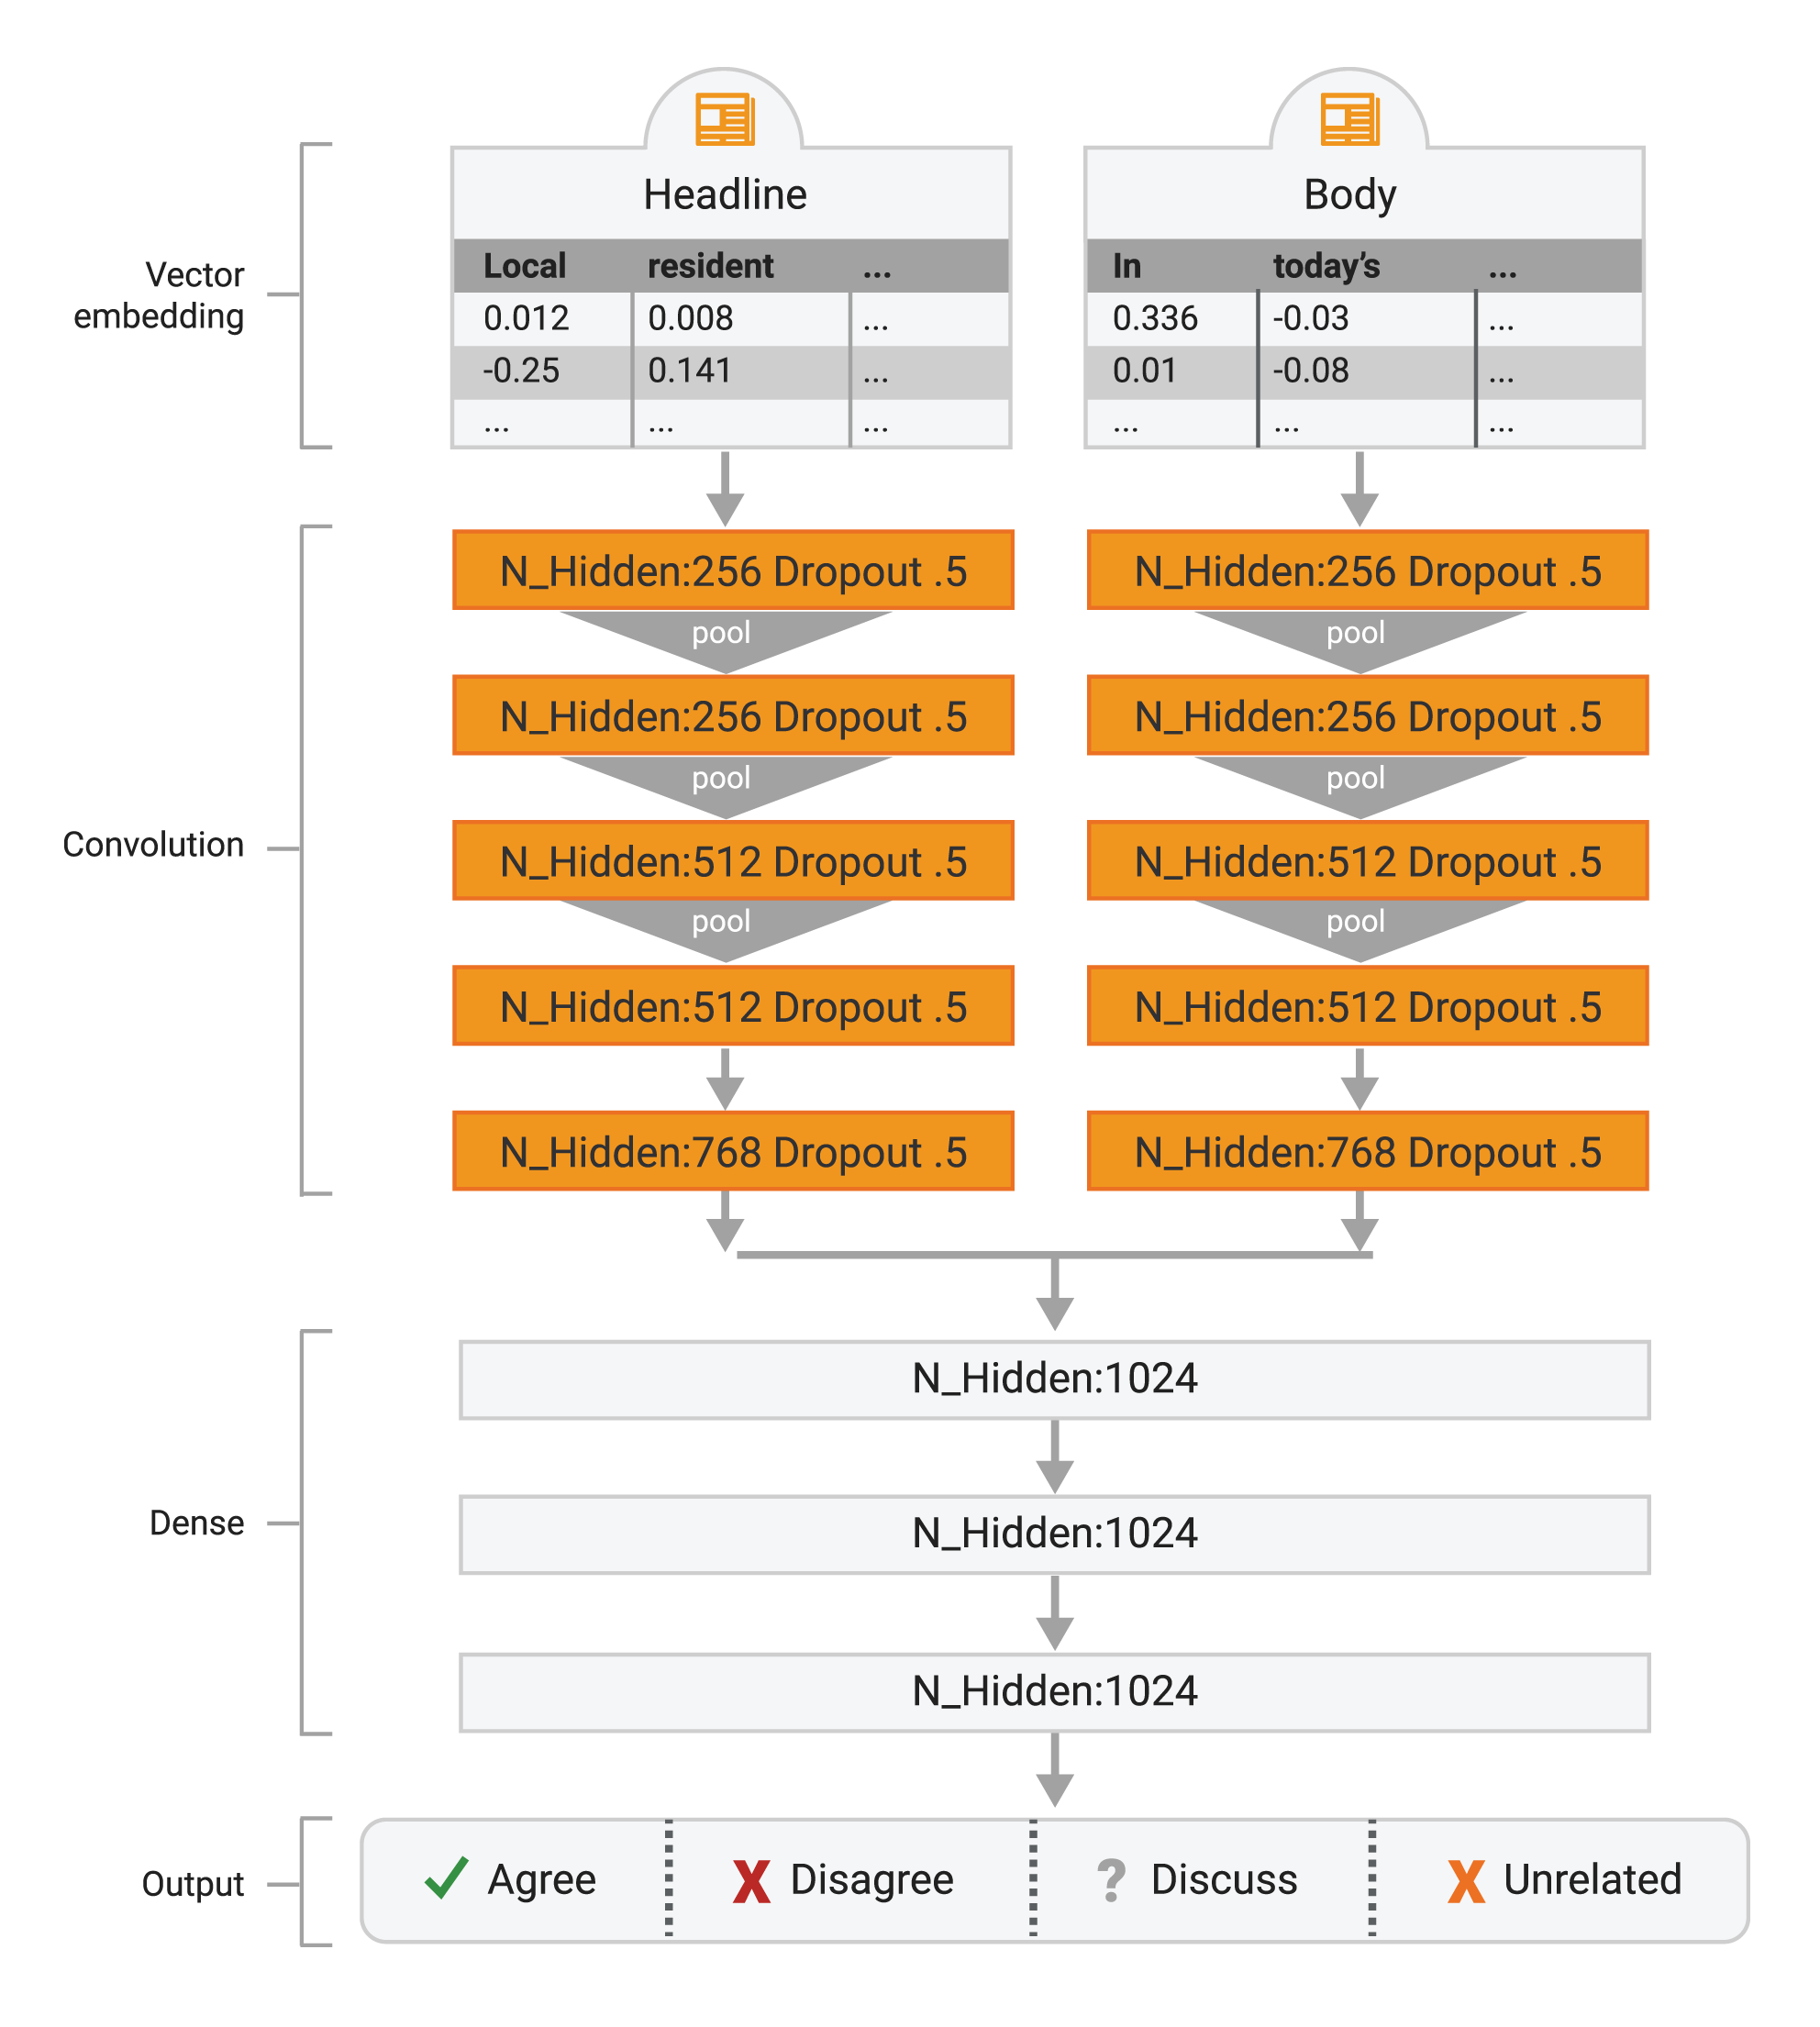
\includegraphics[scale=0.5]{../../img/model/solat_in_the_swen/deep_model_light.png}
 \captionof{figure}{Approche d'apprentissage en profondeur; modèle CNN + MLP.}
 \label{fig1}
\end{center}

Le premier modèle utilisé par l'équipe a plusieurs réseaux de neurones différents utilisés dans l'apprentissage en profondeur.
Ce modèle s'applique à la convolution numérique nette unidimensionnelle (CNN) sur le titre et le corps du texte, en utilisant les vecteurs préchargés de Google News.
Les CNN permettent un calcul parallèle efficace lors de l'exécution.
La sortie de ce CNN est ensuite envoyée à  MLP avec une sortie 4 classes:« agree», « disagree», « discuss» et « unrelated », formés de bout en bout.
Cette architecture de ce modèle fut choisie en raison de sa facilité de mise en œuvre et de son calcul rapide puisque l'on peut compter sur des convolutions au lieu de récurrence.
Il est par contre limité par le fait qu'il ne peut observer le texte qu'une seule fois.


\begin{center}
 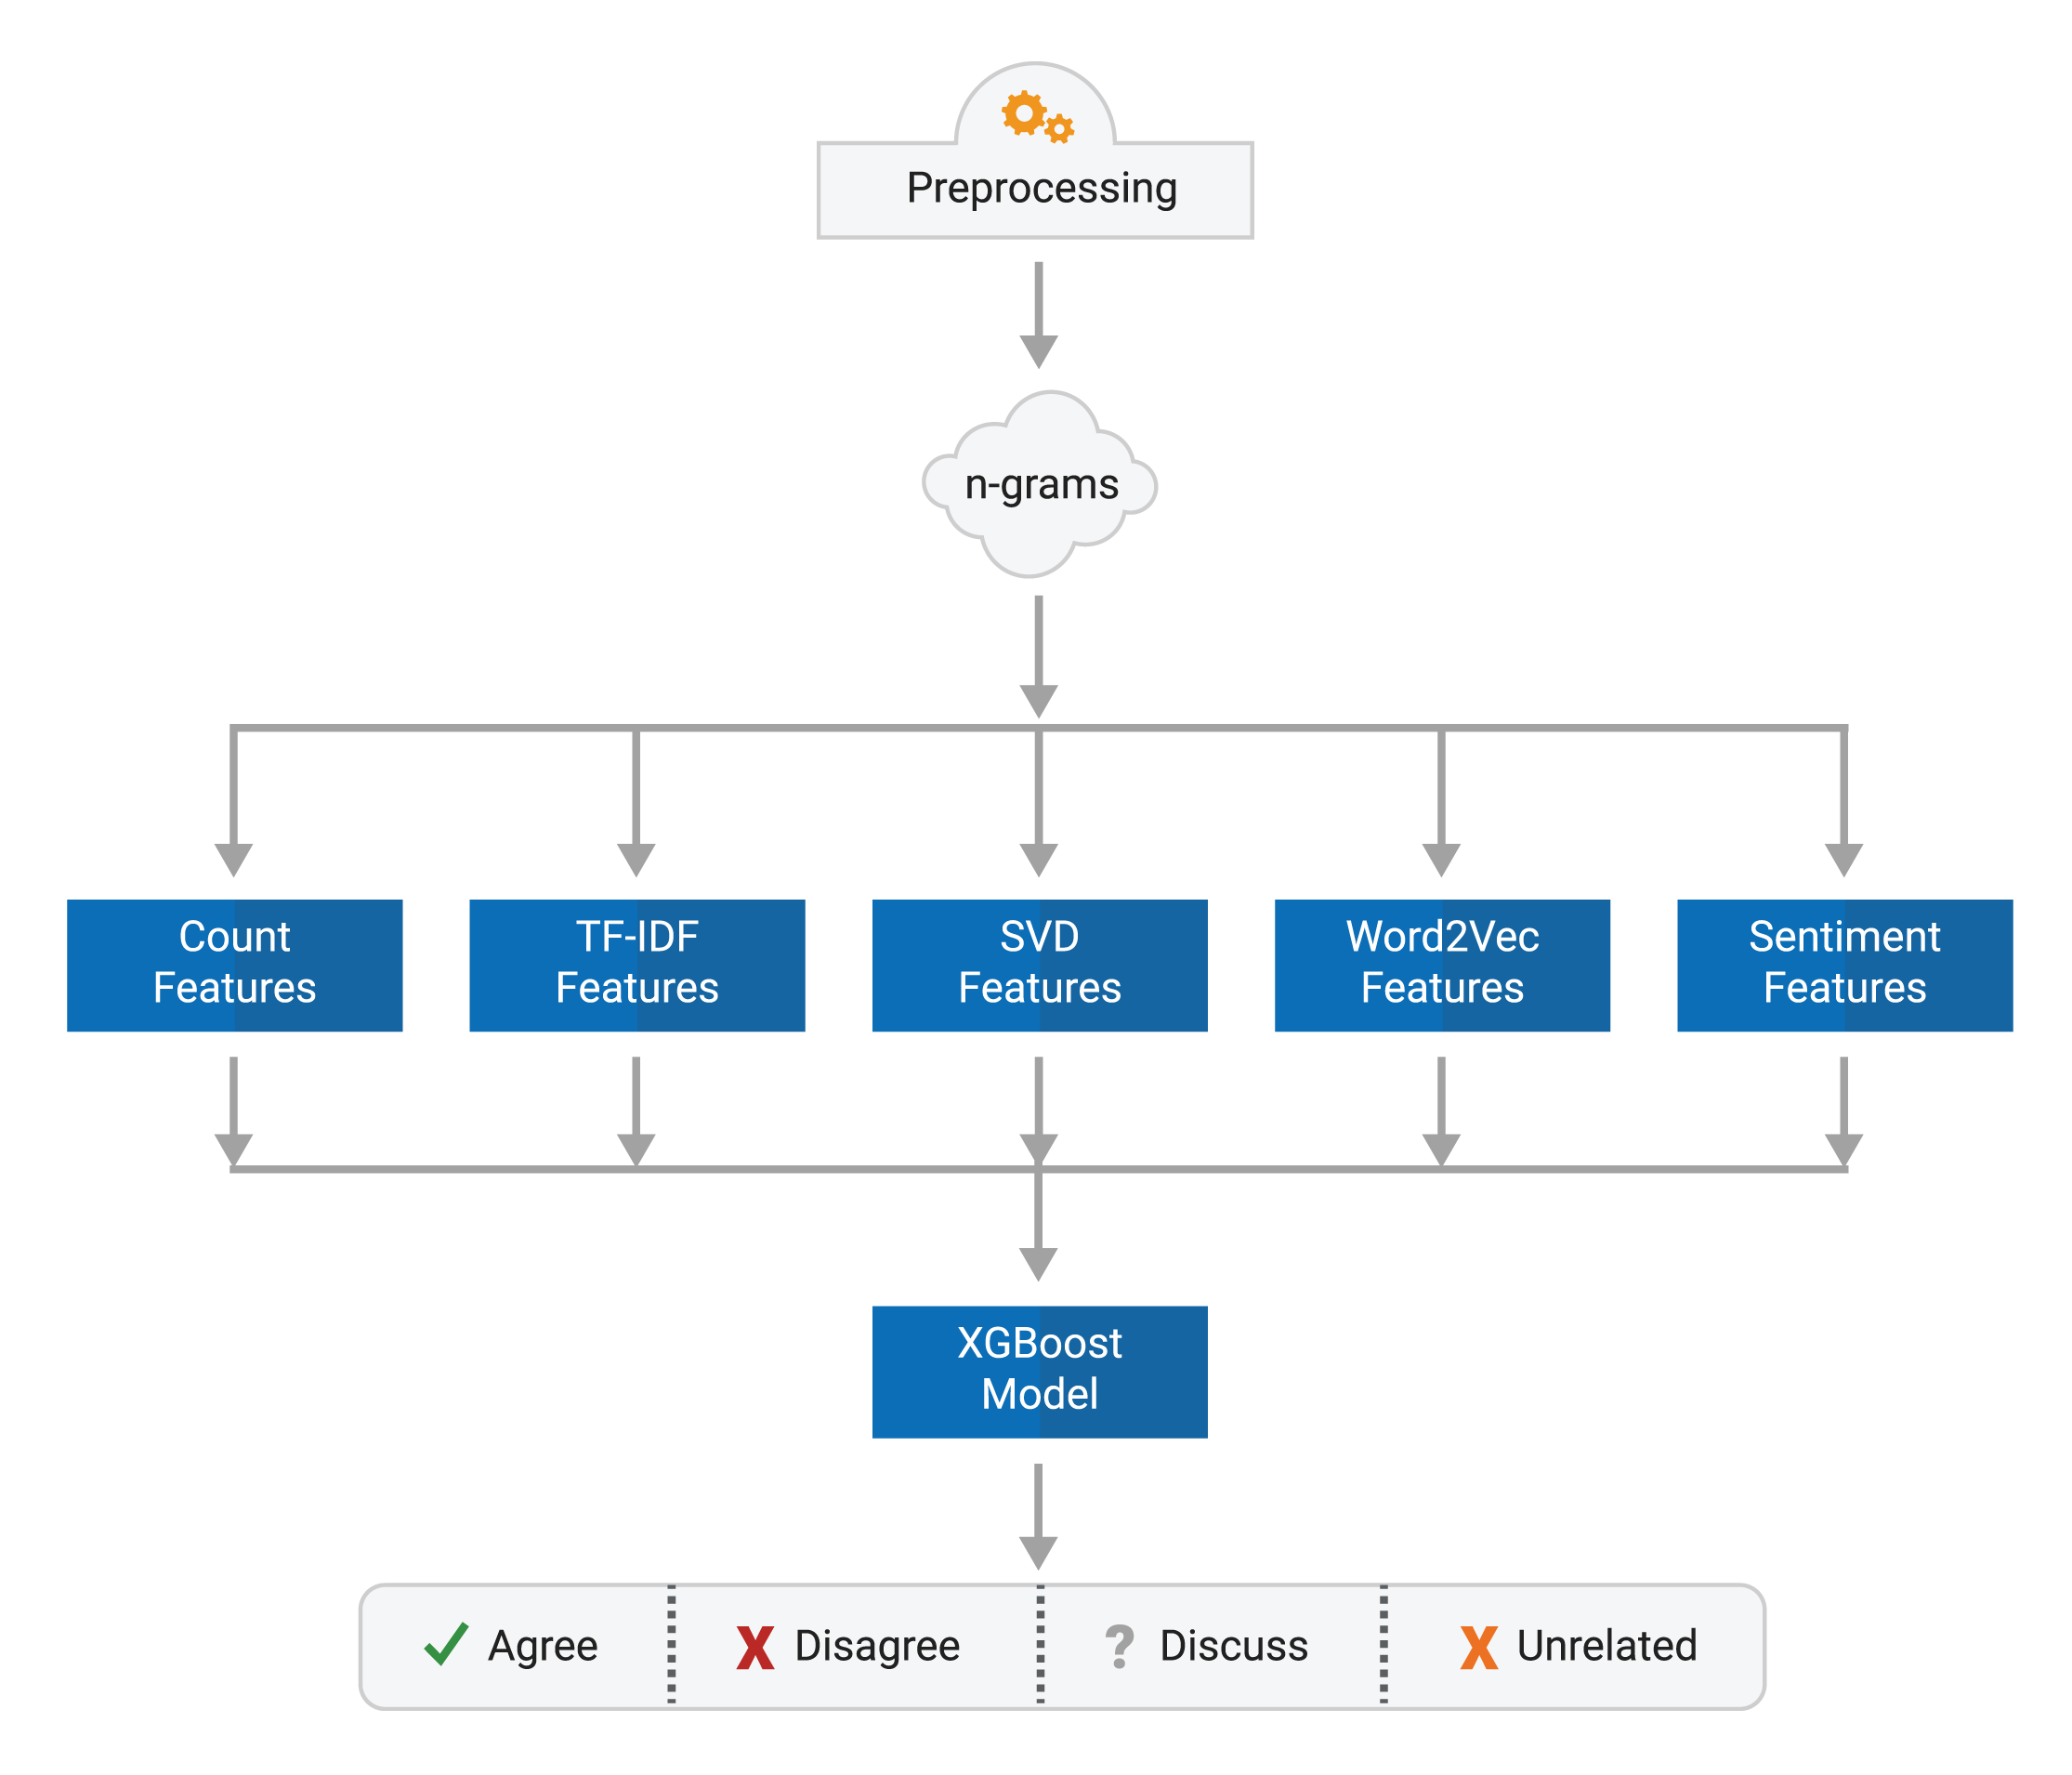
\includegraphics[scale=0.5]{../../img/model/solat_in_the_swen/tree_model_light.png}
 \captionof{figure}{Approche Gradient-Boosted Decision Trees}
 \label{fig2}
\end{center}

L'autre modèle utilisé dans l'ensemble est un modèle d'arbres de décision à gradient d'intensité (GBDT).
Ce modèle introduit peu de caractéristiques textuelles de l'affirmation de rumeurs et du corps de l'article, qui sont ensuite introduites dans le sujet d'un gradient dans la relation entre \textbf{C} et \textbf{E}. Ce modèle basé sur le texte entrainé avec XGBoost utilise plusieurs modules de décision à savoir:
\begin{description}
 \item [Un compteur de trait] pour compter le nombre de trait commun entre le titre et le corps de l'article.
 \item [La méthode de pondération TF-IDF] pour comparer de manière inversé la fréquence relative des mots.
 \item [L'algébre linéaire SVD Features] pour mesurer la similarité entre différents n-grams.
 \item [L'espace vectoriel word2vec] pour comparer le cosinus de similarité entre deux représentation vectorielle.
 \item [Un module Sentiment] utilisant un corpus de mots connotés sentimentalement.
       
\end{description}
Un \textbf{compteur de trait}, pour compter le nombre de trait commun entre le titre et le corps de l'article, la méthode de pondération \textbf{TF-IDF}; pour comparer de manière inversé la fréquence relative des mots, le procédé algebrique linéaire \textbf{SVD Features} pour mesurer la similarité entre différents n-grams, l'espace vectoriel \textbf{word2vec}; pour comparer le cosinus de similarité entre deux représentation vectorielle et un \textbf{module Sentiment} utilisant un corpus de mots connotés sentimentalement.

Les arbres de décision à gradient ont été choisis en raison de la robustesse du modèle par rapport aux différentes échelles des vecteurs caractéristiques.

\subsubsection{Résultats.}
Talos in the swen gagne le FNC avec une score de 9556.50 points donc un score relatif de 82.02\%.


%########################################################################################
%###########Athene (UKP Lab)#############################################################
%########################################################################################


\subsection{Athene (UKP Lab).}
\subsubsection{Méthodologie.}

\begin{center}
 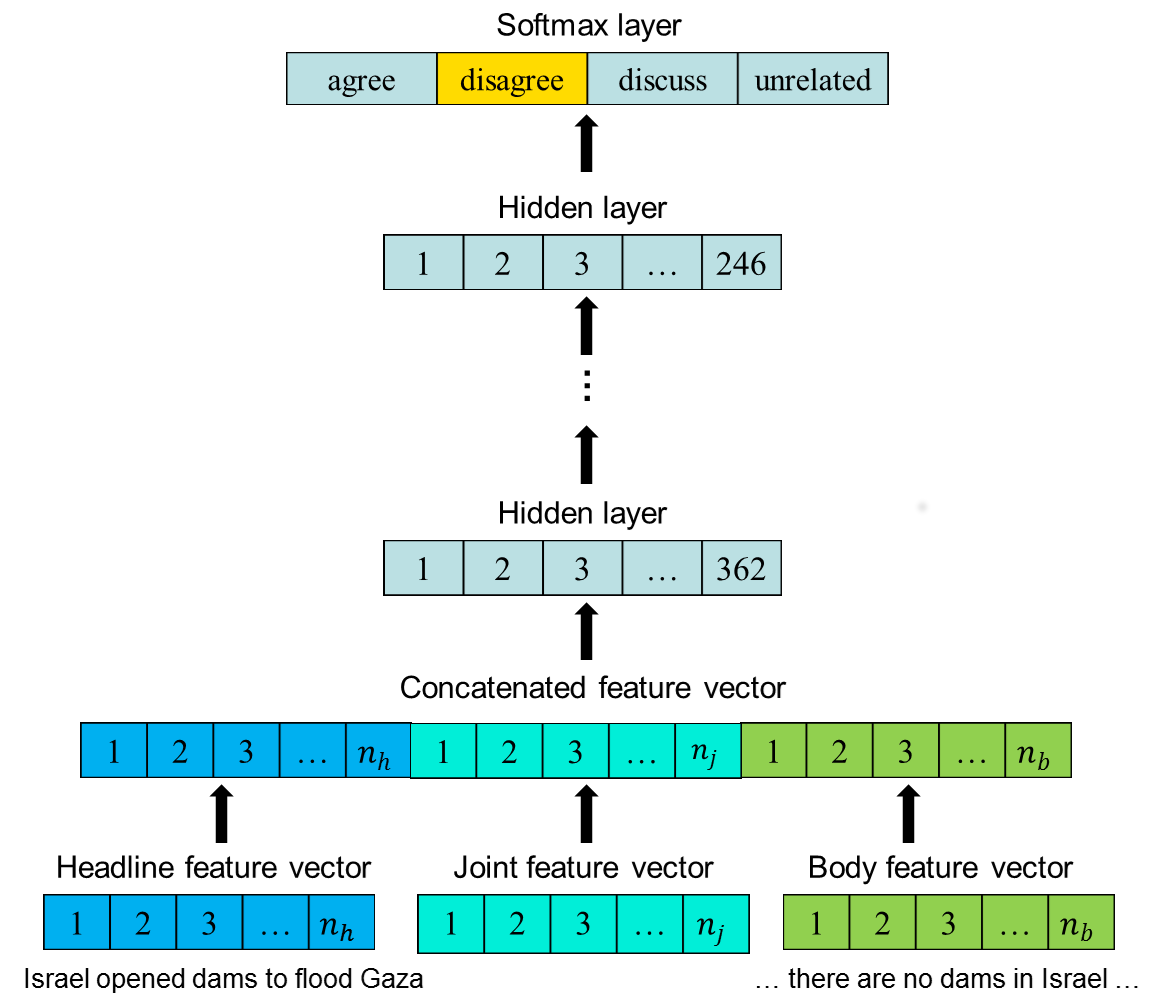
\includegraphics[scale=0.25]{../../img/model/athene/athene_model.png}
 \captionof{figure}{MLP utilisé pour FNC par l'équipe Athene}
 \label{fig3}
\end{center}

Le MLP proposé par Richard Davis et Chris Proctor (organisateurs de FNC) a été le point de départ pour le développement du
système final d'Athene.
La structure du système a été optimisée pour les
caractéristiques par une recherche aléatoire par laquelle les hyper-paramètres ont
été ajusté.
La structure du modèle qui en résulte est illustrée ci-dessus en résumé, car 5 des 7 couches cachées sont ignorées.

Le preprocessing d'Athene utilise différents traits, à savoir: les Bag of Words sur les uni-grams, les matrices de factorisations non-négatives, l'indexation et l'analyses latente sémantique (LSA, LSI) et la détection de paraphrase basé sur le recouvrement de mots (avec word2vec).

La vectorisation des informations se passe en trois étape la vectorisation des données préprocessées de \textbf{C} puis de \textbf{E} et la création d'un vecteur joint des dimension se recoupant dans les deux précédents vecteurs.
Ces trois vecteurs sont alors concaténés en un seul pour former une entrée.

Le modèle final rassemble cinq MLP initialisés de manière aléatoire, qui donnent leurs sorties à un seul MLP qui va faire le vote de la classes à attribuer à partir des autres MLP.
\subsubsection{Résultats}
Athene arrive deuxième au classement du FNC avec une score de 9550.75 points donc un score relatif de 81.97\%.

%########################################################################################
%###########UCL Machine reading##########################################################
%########################################################################################

\subsection{UCL Machine reading.}
\subsubsection{Méthodologie.}
\begin{center}
 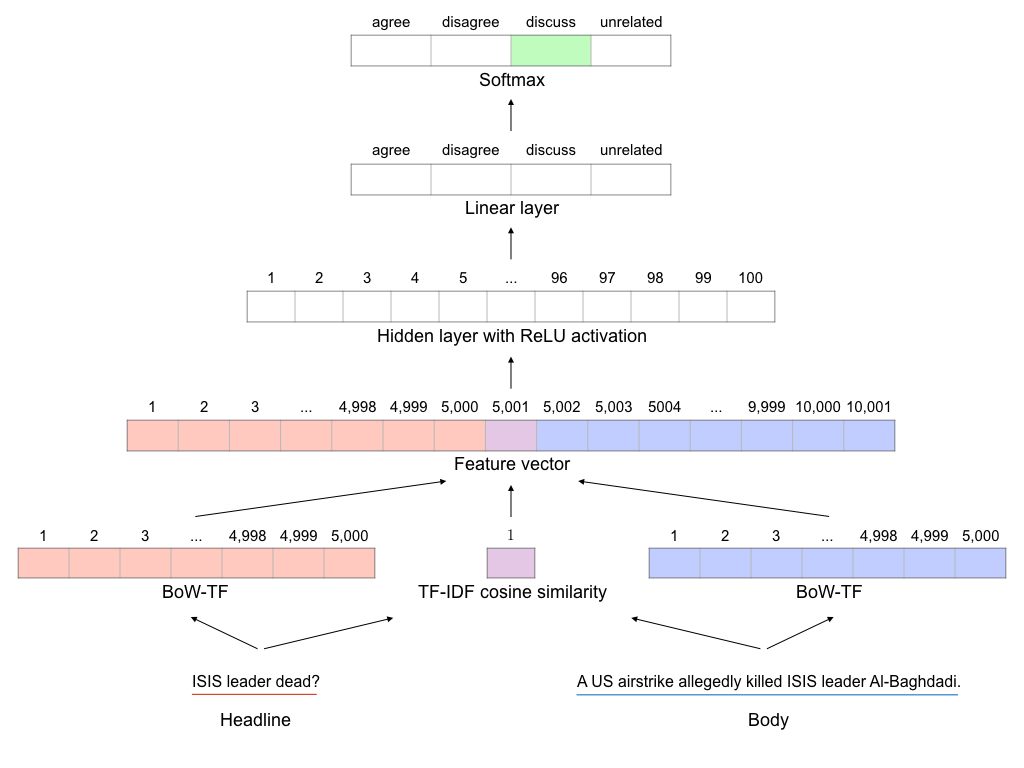
\includegraphics[scale=0.35]{../../img/model/uclmr/uclmr_model.png}
 \captionof{figure}{Schéma du modèle de l'UCLMR.}
 \label{fig4}
\end{center}
UCL-MR est juste un MLP (plutot simple par rapport aux autres solutions) entrainé sur les unigrams et une utilisation astucieuse du TF-IDF.

UCL utilise deux représentations simples des mots avec BoW pour les entrées de texte: fréquence de terme (TF) pour représenter l'affirmation \textbf{C} et le corps de l'article \textbf{E} et l'inverse de la fréquence de la fréquence du document (TF-IDF) pour calculer le cosinus de similarité entre \textbf{E} et \textbf{C}.

Ainsi les vecteurs d'entrée contiennent ces trois vecteurs composites.
Les vecteurs passent dans une seule couche d'entrée de 100 perceptrons avec une activation ReLU.
Puis une couche linear pour donner une valeur à chacune des classes.
Puis un softmax pour sortir la classe dominante.

UCL-MR utilise juste un MLP mais avec des paramètres très optimisés.
Nous ne détaillerons pas ici les paramètres d'implémentation qui se retrouvent dans leur publication.
\subsubsection{Résultats.}
UCL-MR arrive troisième au classement du FNC avec une score de 9521.50 points donc un score relatif de 81.72\%.

\subsection{Discussion comparative des modèles et des résultats.}
% tableau de comparaison des score
\begin{center}
 \begin{tabular}{| c || c | c | }
  \hline
  \textbf{Équipes}  & \textbf{Scores bruts} & \textbf{Scores relatifs} \\
  \hline
  Talos in the Swen & 9556.50               & 82.02\%                  \\
  Athene            & 9550.75               & 81.97\%                  \\
  UCLMR             & 9521.50               & 81.72\%                  \\
  \hline
 \end{tabular}
 \captionof{table}{Résultats ordonnés de la FNC.}
\end{center}

Comme l'a dit Dean Domerleau (organisateur) en parlant de ce tableau de résultats: « Ce que tout cela signifie, c'est que les meilleures équipes se sont très bien débrouillées, mais il y a certainement encore place pour l'amélioration!».
En effet on pourrait pousser plus loin les sytèmes pour que ceux-ci nous donnent de meilleurs résultats.
Mais qu'il n'y ait pas de percée d'une équipe dans le tableau des scores, et le fait que très peu d'équipes on fait mieux que la baseline, montrent que cette tâche est difficile.

De plus un système complexe comme celui de Talos sensé être explicatif sur les traits pertinents ne se démarque que de 0,3 points du système d'UCLMR très peu explicatif mais bien otpimisé, qui reste une boîte noire au niveau de la sélection des paramètres.
On revient à un modèle régréssif qui est simple et qui explique beaucoup avec peu.
Mais cela donne une compréhension minime du phènomène.
Ou peut être le système d'UCLMR est surévalué pour cette ensemble de données.
En ce qui concerne Athene les résultats sont sensiblement les mêmes que Talos.
La complexité de leur modèle est aussi fait à partir d'apprentissages automatisés, certes moins complexe que Talos mais qui reste quand même un modèle avec des systèmes concurents.

Ce qu'il faudrait faire, c'est de comparer les outputs de chaque système et voir comment ils trient les classes \textbf{related}.
Ainsi on pourait faire des recoupements sur les données.
Cela permettrait de constater ce que les différents systèmes font à l'identique et ce qu'ils font différemments.
On en déterminerait les traits et les architectures de modèle relatifs aux classes de données.

C'est ce que je me propose de faire dans la première section de la partie 3 de ce mémoire.
Dans le but ensuite d'apporter une contribution originale à ce problème en partant des systèmes déjà réalisés.


\chapter{Un challenge; des tentatives!}

\section{Analyse des résultats des participants et création d'hypothèses.}
Dans cette troisième partie nous tentons de faire une analyse d'erreurs
comparative des participants de la FNC. Nous avons reproduit les résultats de
tous les participants\footnote{À l'exeption de Talos in the Swen qui ont laissé
 une copie de leur CSV de leurs résultats, pour leurs deux modèles sur leur
 répertoire Github.}.
\subsection{Un aperçu de l'ensemble de test.}
\begin{center}

 \begin{tabular}{ r | c c c c | c}
  Stance      & unrelated & agree  & disagree & discuss &          
  Somme                                                            \\
  \hline
  Nombre      & 18349     & 1903   & 697      & 4464    & 25413    \\
  Pourcentage & 72.20\%   & 7.48\% & 2.74\%   & 17.56\% & 100\%    \\
  Score FNC   & 4587.25   & 1903   & 697      & 4464    & 11651.25 \\
 \end{tabular}
 \captionof{table}{Répartiotion des données dans l'ensembe de test.}
\end{center}

Il y a 7064 points à marquer avec les \textit{Related} et seulement 4587.25 points avec les \textit{Unrelated}.
Ainsi comme nous l'avions vu précédement trouvé un \textit{Related} rapporte 4 fois plus de points que trouvé un \textit{Unrelated}.

Afin de produire des hypothèses non-biaisées  \footnote{Du moins des hypothèses qui ne soient pas ajustées totalement à l'ensemble de test final.}, nous allons faire des observations des résultats des différents modèles sur 80\% des entrées de l'ensemble de test.

\begin{center}
 \begin{tabular}{ r | c c c c | c}
  Stance      & unrelated & agree  & disagree & discuss &        
  Somme                                                          \\
  \hline
  Nombre      & 14662     & 1568   & 550      & 3550    & 20330  \\
  Pourcentage & 72.12\%   & 7.71\% & 2.70\%   & 17.46\% & 100\%  \\
  Score FNC   & 3665.5    & 1568   & 550      & 3550    & 9333.5 \\
 \end{tabular}
 \captionof{table}{Répartition des données dans l'ensembe de test à 80\%.}
\end{center}

Le corpus de test étant partiellement ordonné nous avons retiré les 20\% de manière ordonnée\footnote{En effet, nous avons retiré toutes les entrées dont l'indice été divisible par 5 ou 10} aussi.

\section{Les résultats et les scores des participants.}
Ici nous présentons les différents résultats des modèles de chaque participant sur notre ensemble de test à 80\%.
Notez que les tables de confusions ont horizontalement les labels de vérité et verticalement les prédictions.
Nous présentons les participants du premiers au derniers selon le score FNC.
\subsection{Talos in the Swen.}
\begin{center}
 \begin{tabular}{ r | c c c c | c }
  \multicolumn{6}{c}{Talos Complet}                          \\
  \hline
            & agree & disagree & discuss & unrelated & Somme \\
  \hline
  agree     & 927   & 11       & 478     & 152       & 1568  \\
  disagree  & 217   & 8        & 235     & 90        & 550   \\
  discuss   & 661   & 5        & 2700    & 184       & 3550  \\
  unrelated & 26    & 0        & 172     & 14464     & 14662 \\
  \hline
  Somme     & 1831  & 24       & 3585    & 14890     & 20330 \\
 \end{tabular}
 \captionof{table}{Table de confusion du modèle: Talos Complet}
\end{center}

On remarque que la classe \textbf{disagree} est largement sous-représentée. Cette classe est aussi sous-représentée dans l'ensemble d'entrainement. Ce qui explique potentiellement pourquoi nous ne détectons pas ces traits distinctifs.
\begin{center}
 \begin{tabular}{ r | c c c c }
  \multicolumn{5}{c}{Talos Complet}                                              \\
  Mesure          & agree                       & disagree & discuss & unrelated \\
  \hline
  Précision       & 0.59                        & 0.01     & 0.76    & 0.99      \\
  Rappel          & 0.51                        & 0.33     & 0.75    & 0.97      \\
  F1score         & 0.55                        & 0.03     & 0.76    & 0.98      \\
  \hline
  \hline
  Exactitude      & \multicolumn{4}{c}{89.03}                                    \\
  Score FNC       & \multicolumn{4}{c}{7652.75}                                  \\
  Pourcentage FNC & \multicolumn{4}{c}{81.99}                                    \\
 \end{tabular}
 \captionof{table}{Mesures pour le modèle: Talos Complet}
\end{center}

Bien que Talos in the Swen ait remporté la 1er place de la FNC, l'exactitudes et les scores ci-dessus ne sont pas les maximaux.

%%%%%%%%%%%%%%%%%%%%%%%%%%%%%%%%%%%%%%%%%%%%%%%%%%%%%%%%%%%%%%%%%%%%%%%


\subsubsection{Les sous-modèles de Talos in the Swen.}
\paragraph{Sous-modèle arborescent de Talos in the Swen}
Les sous-modèles de Talos n'ont pas eu de soumission à la FNC mais ils sont quand même intéressants à étudier car ils expliquent les résultats et les biais du modèles.

\begin{center}
 \begin{tabular}{ r | c c c c | c }
  \multicolumn{6}{c}{Talos Arborescent}                      \\
  \hline
            & agree & disagree & discuss & unrelated & Somme \\
  \hline
  agree     & 807   & 0        & 690     & 71        & 1568  \\
  disagree  & 147   & 1        & 334     & 68        & 550   \\
  discuss   & 500   & 1        & 2902    & 147       & 3550  \\
  unrelated & 16    & 0        & 160     & 14486     & 14662 \\
  \hline
  Somme     & 1470  & 2        & 4086    & 14772     & 20330 \\
 \end{tabular}
 \captionof{table}{Table de confusion du modèle: Talos Arborescent}
\end{center}



On voit d'où le modèle principal tient son aversion du label \textbf{disagree}.

\begin{center}
 \begin{tabular}{ r | c c c c }
  \multicolumn{5}{c}{Talos Arborescent}                                         \\
  Mesure          & agree                      & disagree & discuss & unrelated \\
  \hline
  Précision       & 0.51                       & 0.0      & 0.82    & 0.99      \\
  Rappel          & 0.55                       & 0.5      & 0.71    & 0.98      \\
  F1score         & 0.53                       & 0.0      & 0.76    & 0.98      \\
  \hline
  \hline
  Exactitude      & \multicolumn{4}{c}{89.5}                                    \\
  Score FNC       & \multicolumn{4}{c}{7749.5}                                  \\
  Pourcentage FNC & \multicolumn{4}{c}{83.03}                                   \\
 \end{tabular}
 \captionof{table}{Mesures pour le modèle: Talos Arborescent}
\end{center}


Ce sous-modèles ne tient pas vraiment compte de la classe \textbf{disagree} mais il a paradoxalement tout de même les plus hauts scores du challenge. En effet si Talos avait proposé uniquement ce modèle il aurait pris encore plus  d'avance par rapport aux autres participants.
%%%%%%%%%%%%%%%%%%%%%%%%%%%%%%%%%%%%%%%%%%
\paragraph{Sous-modèle de Deep Learning de Talos in the Swen}
\begin{center}
 \begin{tabular}{ r | c c c c | c }
  \multicolumn{6}{c}{Talos DeepLearning}                     \\
  \hline
            & agree & disagree & discuss & unrelated & Somme \\
  \hline
  agree     & 911   & 115      & 143     & 399       & 1568  \\
  disagree  & 271   & 62       & 41      & 176       & 550   \\
  discuss   & 1396  & 137      & 1397    & 620       & 3550  \\
  unrelated & 2321  & 449      & 766     & 11126     & 14662 \\
  \hline
  Somme     & 4899  & 763      & 2347    & 12321     & 20330 \\
 \end{tabular}
 \captionof{table}{Table de confusion du modèle: Talos DeepLearning}
\end{center}



Nous voyons clairement que ce sous-modèle vient équilibrer le sous-modèle arborescent. Sa table de confusion montre une tentative d'uniformisation de la classe \textbf{disagree}.
\begin{center}
 \begin{tabular}{ r | c c c c }
  \multicolumn{5}{c}{Talos deep}                                                 \\
  Mesure          & agree                       & disagree & discuss & unrelated \\
  \hline
  Précision       & 0.58                        & 0.11     & 0.39    & 0.76      \\
  Rappel          & 0.19                        & 0.08     & 0.6     & 0.9       \\
  F1score         & 0.28                        & 0.09     & 0.47    & 0.82      \\
  \hline
  \hline
  Exactitude      & \multicolumn{4}{c}{66.38}                                    \\
  Score FNC       & \multicolumn{4}{c}{5677.25}                                  \\
  Pourcentage FNC & \multicolumn{4}{c}{60.83}                                    \\
 \end{tabular}
 \captionof{table}{Mesures pour le modèle: Talos DeepLearning}
\end{center}


Cette uniformisation a pour conséquence que ce sous-modèle est le pire de tous les modèles. Combiné avec le sous-modèle arborescent, il permet d'avoir une augmentation minime de la classe \textbf{disagree} au détriment des autres classes.
%%%%%%%%%%%%%%%%%%%%%%%%%%%%%%%%%%%%%%%%%%%%%%%%%%%%%%%%%%%

\subsection{Le système Athene}


\begin{center}
 \begin{tabular}{ r | c c c c | c }
  \multicolumn{6}{c}{Athene}                                 \\
  \hline
            & agree & disagree & discuss & unrelated & Somme \\
  \hline
  agree     & 709   & 57       & 669     & 133       & 1568  \\
  disagree  & 193   & 56       & 193     & 108       & 550   \\
  discuss   & 388   & 30       & 2853    & 279       & 3550  \\
  unrelated & 16    & 3        & 86      & 14557     & 14662 \\
  \hline
  Somme     & 1306  & 146      & 3801    & 15077     & 20330 \\
 \end{tabular}
 \captionof{table}{Table de confusion du modèle: Athene}
\end{center}



La table de confusion d'Athene ressembe beaucoup à celle de Talos. Ce modèle tente beaucoup plus de labéliser des titres d'articles comme \textbf{diagree}. Mais il a beaucoup plus de mal à distinguer la classe \textbf{discuss} de la classe \textbf{agree}.

\begin{center}
 \begin{tabular}{ r | c c c c }
  \multicolumn{5}{c}{Athene}                                                     \\
  Mesure          & agree                       & disagree & discuss & unrelated \\
  \hline
  Précision       & 0.45                        & 0.1      & 0.8     & 0.99      \\
  Rappel          & 0.54                        & 0.38     & 0.75    & 0.97      \\
  F1score         & 0.49                        & 0.16     & 0.78    & 0.98      \\
  \hline
  \hline
  Exactitude      & \multicolumn{4}{c}{89.4}                                     \\
  Score FNC       & \multicolumn{4}{c}{7639.75}                                  \\
  Pourcentage FNC & \multicolumn{4}{c}{81.85}                                    \\
 \end{tabular}
 \captionof{table}{Mesures pour le modèle: Athene}
\end{center}


Athene a la meilleure exactitude de toute la FNC car elle classe très bien les \textbf{unrelated} (qui ne valent pas beaucoup de points dans le score FNC).


\subsection{UCL Machine Reader}




\begin{center}
 \begin{tabular}{ r | c c c c | c }
  \multicolumn{6}{c}{Uclmr}                                  \\
  \hline
            & agree & disagree & discuss & unrelated & Somme \\
  \hline
  agree     & 697   & 7        & 770     & 94        & 1568  \\
  disagree  & 144   & 37       & 277     & 92        & 550   \\
  discuss   & 424   & 35       & 2882    & 209       & 3550  \\
  unrelated & 44    & 2        & 261     & 14355     & 14662 \\
  \hline
  Somme     & 1309  & 81       & 4190    & 14750     & 20330 \\
 \end{tabular}
 \captionof{table}{Table de confusion du modèle: Uclmr}
\end{center}


Nous observons une tentative d'uniformisation proportionnelle de la table de confusion.
UCLMR sait très bien classé les \textbf{unrelated}. Néanmoins, il manque apparemment de traits pour distinguer les \textbf{agree} des \textbf{discuss}.


\begin{center}
 \begin{tabular}{ r | c c c c }
  \multicolumn{5}{c}{Uclmr}                                                     \\
  Mesure          & agree                      & disagree & discuss & unrelated \\
  \hline
  Précision       & 0.44                       & 0.07     & 0.81    & 0.98      \\
  Rappel          & 0.53                       & 0.46     & 0.69    & 0.97      \\
  F1score         & 0.48                       & 0.12     & 0.74    & 0.98      \\
  \hline
  \hline
  Exactitude      & \multicolumn{4}{c}{88.4}                                    \\
  Score FNC       & \multicolumn{4}{c}{7619.0}                                  \\
  Pourcentage FNC & \multicolumn{4}{c}{81.63}                                   \\
 \end{tabular}
 \captionof{table}{Mesures pour le modèle: Uclmr}
\end{center}

\subsection{Analyses et Hypothèses}
Voici un liste d'hypothéses basée sur nos constatations que nous testerons de vérifier par la suite avec les différents modèles.
Nous voyons clairement une confusion entre la \textbf{agree} et la classe \textbf{discuss}.
Mieux distinguer ces deux classe rapporterait gros Et pourrait faire un différence significative.
La classe \textbf{disagree} est sous-représentée donc quantitativement elle ne rapporte que peu de points.
Le modèls de Talos semble plus robuste que les autres en utilisant l'apprentissage par ensemble (\textit{ensemble learning}).
Utiliser ce type d'apprentissage entre les modèles des participants augmenterait certainement les performances.

\section{Modèles par combinaison:\\ Le vote de majorité}
\subsection{Explication du modèle.}
Comme nous l'avons vu précédement les combinaisons entre les modèles déjà présentés à la FNC peuvent atteindre de hauts résultats.
Notre premier modèle sera un jet naif de combinaisons de deux modèles.
Le vote de majorité se base sur les classes prédites par les modèles des participants pour l'ensemble de test complet.
Ce vote de majorité marche avec un modèle dominant départageant en cas de conflict entre les deux autres modèles assujettis.
La classe la plus voté sera la classe prédite.
Si jamais les trois classes sont toutes différentes alors est choisie la classe donné par le modèle dominant.

\begin{center}
 \begin{tabular}{  c c c || c  }
  \multicolumn{4}{c}{Vote de majorité entre 3 modèles}                          \\
  \hline
  Modèle Dominant  & Modèle assujetti 1 & Modèle assujetti 2 & Classe prédite   \\
  \hline
  \textbf{agree}   & \textbf{agree}     & unrelated          & \textbf{agree}   \\
  disagree         & \textbf{discuss}   & \textbf{discuss}   & \textbf{discuss} \\
  \textbf{discuss} & disagree           & agree              & \textbf{discuss} \\
 \end{tabular}
 \captionof{table}{Exemple du vote de majorité}
\end{center}

Ainsi chaque modèle à tour de rôle peut devenir le modèle dominant.
Ce qui donne les résultats dans la sous-sections suivantes.

\subsection{Les résultats des votes de majorité}
\subsubsection{Dominant: Talos in the swen}

\begin{center}
 \begin{tabular}{ r | c c c c | c }
  \multicolumn{6}{c}{Vote de majorité avec dominant: Talos}  \\
  \hline
            & agree & disagree & discuss & unrelated & Somme \\
  \hline
  agree     & 923   & 13       & 815     & 152       & 1903  \\
  disagree  & 228   & 20       & 321     & 128       & 697   \\
  discuss   & 483   & 4        & 3729    & 248       & 4464  \\
  unrelated & 27    & 0        & 149     & 18173     & 18349 \\
  \hline
  Somme     & 1661  & 37       & 5014    & 18701     & 25413 \\
 \end{tabular}
 \captionof{table}{Table de confusion du modèle}
\end{center}


\begin{center}
 \begin{tabular}{ r | c c c c }
  \multicolumn{5}{c}{Vote de majorité avec dominant: Talos}                      \\
  Mesure          & agree                       & disagree & discuss & unrelated \\
  \hline
  Précision       & 0.49                        & 0.03     & 0.84    & 0.99      \\
  Rappel          & 0.56                        & 0.54     & 0.74    & 0.97      \\
  F1score         & 0.52                        & 0.05     & 0.79    & 0.98      \\
  \hline
  \hline
  Exactitude      & \multicolumn{4}{c}{89.89}                                    \\
  Score FNC       & \multicolumn{4}{c}{9681.25}                                  \\
  Pourcentage FNC & \multicolumn{4}{c}{83.09}                                    \\
 \end{tabular}
 \captionof{table}{Mesures pour le modèle: Vote de majorité Talos}
\end{center}

\subsubsection{Dominant: Athene}

\begin{center}
 \begin{tabular}{ r | c c c c | c }
  \multicolumn{6}{c}{Vote de majorité avec dominant: Athene} \\
  \hline
            & agree & disagree & discuss & unrelated & Somme \\
  \hline
  agree     & 914   & 42       & 809     & 138       & 1903  \\
  disagree  & 213   & 46       & 308     & 130       & 697   \\
  discuss   & 453   & 21       & 3735    & 255       & 4464  \\
  unrelated & 14    & 2        & 148     & 18185     & 18349 \\
  \hline
  Somme     & 1594  & 111      & 5000    & 18708     & 25413 \\
 \end{tabular}
 \captionof{table}{Table de confusion du modèle}
\end{center}



\begin{center}
 \begin{tabular}{ r | c c c c }
  \multicolumn{5}{c}{Vote de majorité avec dominant: Athene}                     \\
  Mesure          & agree                       & disagree & discuss & unrelated \\
  \hline
  Précision       & 0.48                        & 0.07     & 0.84    & 0.99      \\
  Rappel          & 0.57                        & 0.41     & 0.75    & 0.97      \\
  F1score         & 0.52                        & 0.11     & 0.79    & 0.98      \\
  \hline
  \hline
  Exactitude      & \multicolumn{4}{c}{90.03}                                    \\
  Score FNC       & \multicolumn{4}{c}{9702.75}                                  \\
  Pourcentage FNC & \multicolumn{4}{c}{83.28}                                    \\
 \end{tabular}
 \captionof{table}{Mesures pour le modèle: Vote de majorité Athene}
\end{center}
\subsubsection{Dominant: UCL Machine Reader}

\begin{center}
 \begin{tabular}{ r | c c c c | c }
  \multicolumn{6}{c}{Vote de majorité avec dominant: uclmr}  \\
  \hline
            & agree & disagree & discuss & unrelated & Somme \\
  \hline
  agree     & 920   & 13       & 844     & 126       & 1903  \\
  disagree  & 202   & 35       & 339     & 121       & 697   \\
  discuss   & 467   & 26       & 3728    & 243       & 4464  \\
  unrelated & 19    & 1        & 157     & 18172     & 18349 \\
  \hline
  Somme     & 1608  & 75       & 5068    & 18662     & 25413 \\
 \end{tabular}
 \captionof{table}{Table de confusion du modèle}
\end{center}


\begin{center}
 \begin{tabular}{ r | c c c c }
  \multicolumn{5}{c}{Vote de majorité avec dominant: Uclmr}                      \\
  Mesure          & agree                       & disagree & discuss & unrelated \\
  \hline
  Précision       & 0.48                        & 0.05     & 0.84    & 0.99      \\
  Rappel          & 0.57                        & 0.47     & 0.74    & 0.97      \\
  F1score         & 0.52                        & 0.09     & 0.78    & 0.98      \\
  \hline
  \hline
  Exactitude      & \multicolumn{4}{c}{89.93}                                    \\
  Score FNC       & \multicolumn{4}{c}{9698.75}                                  \\
  Pourcentage FNC & \multicolumn{4}{c}{83.24}                                    \\
 \end{tabular}
 \captionof{table}{Mesures pour le modèle: Vote de majorité Uclmr}
\end{center}

\subsubsection{Commentaires sur les résultats du vote de majorité}
Bien que ce modèle d'apprentissage par ensemble semble être le plus naïf; ces résultats sont les plus haut que l'on obtiendra.
On remarque que Athene est le meilleur des modèles dominants.
C'est le modèle qui se trompe le moins en cas de conflit.



\section{Modèles par combinaison: \\ Par moyenne}

\subsection{Modèles utiliseant \textit{50/50 weighted average}}

Pour ce modèle, deux sous-modèles  génèreront des probalités de label pour chaque entrée.
Nous nous s'inspirerons de la méthode d'unification de Talos.
Nous utiliserons donc aussi un \textit{50/50 weighted average} pour combiner les résultats.
Ainsi chaque sous-modèles produira un vecteurs de dimension 4 pour chaque labels.
Chaque couple de même dimensions passera par un \textit{50/50 weighted average}.
Le maximum des 4 résultats des moyennes indiquera la classe prédite pour l'entrée.

Notre première architecture utilisera le sous-modèle arborescent de Talos et le modèle de UCL Machine Reader.
Nous appelerons ce modèles « mixte UCLMR/Talos TF-Idf».

Notre deuxième architecture utilisera aussi le sous-modèle arborescent de Talos et le modèle de UCL Machine Reader mais dans cette version le sous modèle arborescent de Talos n'utiliseras pas son de TF-Idf. La raison est que le système de UCL utilise déjà et uniquement ces traits-là. Ainsi pour augmenter la différence entre les résultats des deux sous-modèles, nous décidons de retirer ce module. De plus il sera entrainé seleument sur les données d'entraînement pour créer son espace sémantique\footnote{En effet dans la version originale du modèle lors de la création de l'espace sémantique les données de test viennent augmentées les données d'entrainement. Cela a pour conséquence que le modèle ait déjà vu les données de test lors de son entrainement. Mais ne nous méprenons pas cela est autorisé dans le réglement de la FNC même si cela est assez questionnable.}.
Nous appelerons ce modèles « mixte UCLMR/Talos sans TF-Idf».


\subsection{Résultats}

\subsubsection{Modèles mixte UCLMR/Talos TF-Idf}

\begin{center}
 \begin{tabular}{ r | c c c c | c }
  \multicolumn{6}{c}{Mixte UCLMR/Talos TF-Idf}               \\
  \hline
            & agree & disagree & discuss & unrelated & Somme \\
  \hline
  agree     & 963   & 0        & 819     & 121       & 1903  \\
  disagree  & 198   & 1        & 377     & 121       & 697   \\
  discuss   & 606   & 3        & 3612    & 243       & 4464  \\
  unrelated & 21    & 0        & 166     & 18162     & 18349 \\
  \hline
  Somme     & 1788  & 4        & 4974    & 18647     & 25413 \\
 \end{tabular}
 \captionof{table}{Table de confusion du modèle: Mixte UCLMR/Talos TF-Idf}
\end{center}
Cette table de confusion ressemble beaucoup à celle de Talos dans l'analyse sur 80\% du corpus.
Sans surprise, la classe disagree n'est pas améliorée.
Par contre, les classes agree, discuss et unrelated sont légèrement augmentées.

\begin{center}
 \begin{tabular}{ r | c c c c }
  \multicolumn{5}{c}{Mixte UCLMR/Talos TF-Idf}                                   \\
  Mesure          & agree                       & disagree & discuss & unrelated \\
  \hline
  Précision       & 0.51                        & 0.0      & 0.81    & 0.99      \\
  Rappel          & 0.54                        & 0.25     & 0.73    & 0.97      \\
  F1score         & 0.52                        & 0.0      & 0.77    & 0.98      \\
  \hline
  \hline
  Exactitude      & \multicolumn{4}{c}{89.47}                                    \\
  Score FNC       & \multicolumn{4}{c}{9617.25}                                  \\
  Pourcentage FNC & \multicolumn{4}{c}{82.54}                                    \\
 \end{tabular}
 \captionof{table}{Mesures pour le modèle: Mixte UCLMR/Talos TF-Idf}
\end{center}
Nous constatons un gain de 0.52\% par rapport au meilleur des systèmes de la FNC.
Ceci est peu mais montre une amélioration minime de la précision de la classe agree et de la classe discuss.
La classe disagree est encore négligée par le modèle arborescent de Talos.
En conséquence, le modèle UCLMR biaisé par Talos ne permet pas d'améliorer la précision de la classe disagree.


\subsubsection{Modéles mixte UCLMR/Talos sans TF-Idf}
\begin{center}
 \begin{tabular}{ r | c c c c | c }
  \multicolumn{6}{c}{ixte UCLMR/Talos sans TF-Idf}           \\
  \hline
            & agree & disagree & discuss & unrelated & Somme \\
  \hline
  agree     & 1002  & 0        & 776     & 125       & 1903  \\
  disagree  & 216   & 1        & 357     & 123       & 697   \\
  discuss   & 602   & 2        & 3596    & 264       & 4464  \\
  unrelated & 16    & 0        & 149     & 18184     & 18349 \\
  \hline
  Somme     & 1836  & 3        & 4878    & 18696     & 25413 \\
 \end{tabular}
 \captionof{table}{Table de confusion du modèle: mixte UCLMR/Talos sans TF-Idf}
\end{center}

Par rapport au modèle mixte UCLMR/Talos TF-Idf, ce modèle améliore la classe des \textbf{agree} d'une quarantaine d'entrée.
C'est certes un avantage minime, qui n'en reste pas moins surprenant.
En effet le modèle avec TF-Idf a un espace sémantique plus exhaustif et plus proche de l'ensemble de test.



\begin{center}
 \begin{tabular}{ r | c c c c }
  \multicolumn{5}{c}{Mixte UCLMR/Talos sans TF-Idf}                              \\
  Mesure          & agree                       & disagree & discuss & unrelated \\
  \hline
  Précision       & 0.53                        & 0.0      & 0.81    & 0.99      \\
  Rappel          & 0.55                        & 0.33     & 0.74    & 0.97      \\
  F1score         & 0.54                        & 0.0      & 0.77    & 0.98      \\
  \hline
  \hline
  Exactitude      & \multicolumn{4}{c}{89.65}                                    \\
  Score FNC       & \multicolumn{4}{c}{9633.25}                                  \\
  Pourcentage FNC & \multicolumn{4}{c}{82.68}                                    \\
 \end{tabular}
 \captionof{table}{Mesures pour le modèle: mixte UCLMR/Talos sans TF-Idf}
\end{center}

Certes l'avantagesur le modèle précédent n'est que de 0.16\% pour les pourcentage FNC.
Peut-être montrons-nous qu'un espace sémantique simplement formé avec l'ensemble d'entrainement est suffisant.



\section{Apprentissage par ensemble: \\ Avec \textit{Single Layer Learner}}
\subsection{Explication du modèle}
Une des meilleurs manière \textit{a priori} de déterminer une classe à partir d'une liste de probabilité est certainement d'utiliser un couche neuronale.
Ainsi nous avons créer avec le framework Keras un \textit{Single Layer Learner}.
Celui-ci dispose d'un couche d'entrée de la longueur de nos vecteurs d'entrainement, d'un couche de 32 unités d'apprentissage et d'une couche de sortie de 4 unités, une par label.
Afin de produire les vecteurs d'entrainement nous avons utiliser l'intégralité du corpus d'entrainement.
Chaque dixième des vecteurs on était produits par les 90\% restant du corpus.
Les données qui ont servi à produire les vecteurs d'entraînement sont les vecteurs concaténé du modèle Mixte UCLMR/Talos sans TF-Idf.
Nous nommerons ce modèle Mixte UCLMR/Talos sans TF-Idf SLL.

\subsubsection{Code du modèle}
\begin{lstlisting}[language=Python]

  import numpy as np
  import keras
  from keras.models import Sequential
  from keras.layers import Dense, Activation
  import tensorflow as tf


  def create_trained_nn(vecs_train, labels_train, epochs=50):
      """Create a trained neural network model."""
      input_dim = vecs_train.shape[1]
      model = Sequential()
      model.add(Dense(units=32, input_dim=input_dim))
      model.add(Activation('relu'))
      model.add(Dense(units=4))
      model.add(Activation('softmax'))
      model.compile(loss='sparse_categorical_crossentropy',
                    optimizer='sgd',
                    metrics=['accuracy'])
      model.fit(vecs_train, labels_train, epochs=epochs,
                batch_size=32)

      return model
\end{lstlisting}



\subsection{Résultats}
\begin{center}
 \begin{tabular}{ r | c c c c | c }
  \multicolumn{6}{c}{Mixte UCLMR/Talos sans TF-Idf SLL}      \\
  \hline
            & agree & disagree & discuss & unrelated & Somme \\
  \hline
  agree     & 1059  & 3        & 729     & 112       & 1903  \\
  disagree  & 253   & 14       & 323     & 107       & 697   \\
  discuss   & 684   & 7        & 3530    & 243       & 4464  \\
  unrelated & 45    & 0        & 288     & 18016     & 18349 \\
  \hline
  Somme     & 2041  & 24       & 4870    & 18478     & 25413 \\
 \end{tabular}
 \captionof{table}{Table de confusion du modèle: Mixte UCLMR/Talos sans TF-Idf SLL}
\end{center}


\begin{center}
 \begin{tabular}{ r | c c c c }
  \multicolumn{5}{c}{Mixte UCLMR/Talos sans TF-Idf SLL}                          \\
  Mesure          & agree                       & disagree & discuss & unrelated \\
  \hline
  Précision       & 0.56                        & 0.02     & 0.79    & 0.98      \\
  Rappel          & 0.52                        & 0.58     & 0.72    & 0.97      \\
  F1score         & 0.54                        & 0.04     & 0.76    & 0.98      \\
  \hline
  \hline
  Exactitude      & \multicolumn{4}{c}{89.01}                                    \\
  Score FNC       & \multicolumn{4}{c}{9606.75}                                  \\
  Pourcentage FNC & \multicolumn{4}{c}{82.45}                                    \\
 \end{tabular}
 \captionof{table}{Mesures pour le modèle: Mixte UCLMR/Talos sans TF-Idf SLL}
\end{center}

Etonnamment ce modèle a de moins bons résultats que le modèle précédent.
Même en changeant les paramètres d'apprentissage (nombre d'unités d'apprentissage ou nombre de récusrion) le modèle n'excéde pas le précédents.
\section{Discussions}

Notre objectif dans ce troisième chapitre était de proposer des améliorations aux systèmes présentés à la \textit{Fake News Challenge}. Sur la diversité des hypothèses et des tests effectués nous observons qu'il n'y a très peu de systèmes qui dépassent la baseline que l'on s'était fixé (à savoir les résultats de Solat in the swen).

Rappelons que nous avons utilisé trois méthodes combinaison : le vote de majorité, la moyenne pondérée à 50/50 et finalement une méthode d' apprentissage d'ensemble avec une couche neuronalle apprenante.

Nous avons bien vérifié une de nos hypothèses celle qui disait qu'en combinant les résultats de plusieurs systèmes gagnant de la fnc on obtiendrait de meilleurs résultats.
Par contre les résultats nous donnent une bonne leçon d'humilité en ce que nos modèles les plus complexes n'ont pas eu les meilleurs résultats.
En effet le vote de majorité ressort grand gagnant de nos améliorations alors que c'est le système le plus simple et naïf.
A posteriori nous expliquons son succès du fait que c'est le modèle qui dispose le plus de ressources par rapport aux autres. En effet, nos autres modèles de combinaison ou notre modèle d'apprentissage par ensemble ne se base que sur les résultats de deux sous-modèles gagnants, alors que le vote de majorité dispose des résultats de tous les participants gagnants.

Ainsi le modèle de vote de majorité où le système Athene est dominant dépasse notre baseline de 1.26 avec le score de 83,28 au pourcentage fnc.
Nous regrettons, en revanche, la difficulté d'accessibilité du code du système d'Athene au profane. Pour cette raison nous n'avons pas pu produire des probabilités de labels que nos autres modèles utilisent. Ceci est l'explication de l'absence deux moyennes ou d'apprentissage d'ensemble entre Athene et les autres participants.

Nous regrettons aussi de ne pas avoir réussi à utiliser correctement le module TF-IDF du modèle Solat in the swen.
Cela a créé plus de variable indépendante pour nos modèles de moyenne et notre modèle d'apprentissage d'ensemble.
C'est donc moins partique pour la comparaison de modèle.

Notre autre hypothèse : « mieux distinguer les labels agree et discuss améliore les résultats» ne fut pas vérifiée de manière indidrecte.
En effet nous regrettons aussi de ne pas avoir utilisé plus de technologie du traitement du langage afin de mieux faire cette distinction.
Mais à vrai dire nous n'étions pas sur de quelle voie emprunter. Les systèmes gagnants ont explorer de manière assez exhaustive les technologies pertinentes.
Ils ont montré ce qui valait la peine de ce qui était délétère.
Prétendre à proposer des traits non significatif n'était pas notre but.
C'est pourquoi nous nous sommes concentrés sur des combinaisons de système.
Mais si par le futur il venait à y avoir une découverte de très plus significative que les présents, ces systèmes ne demanderaient qu'à être amélioré.

Nous sommes aussi rendu compte que entraîner les systèmes sur les headlines de test ne changez pas beaucoup l'espace sémantique des classifieurs. Les résultats étant assez proche entraîner avec ou sans.

\chapter{Conclusions}


Dans ce mémoire nous avons vu ce qu'était donc une \textit{Fake News} ce phénomène nouveau d'informations volontièrement trompeuses qui pullulent et se reproduisent sur le web. Nous avons décrit les origines leur mode de fonctionnement et leur utilisation. Entre autres nous avons vu à quel point elles peuvent être dangereuses utilisé à des fins autoritaire. Nous avons donc proposé une méthode manuelle pour s'en protéger de manière individuelle et éducative. Ensuite nous sommes allés voir les systèmes informatiques préliminaires de détection de \textit{Fake News}. Labelliser comme vrai/faux est pour le moment impossible, du fait du manques cruel de corpus d'entrainement pour ce type de tâches. Nous nous sommes donc rabattu sur les technologies de traitement de langage qui pourrait potentiellement aider à créer un classifieur \textit{Fake News}/true news par le futur. Ainsi nous avons présenté la détection de position. Nous sommes familiarisé avec le concept avec la tâche 6 semeval 2016 puis nous nous sommes rapprochés de notre but en expliquant la \textit{Fake News Challenge}. Nous avons discuté les différents résultats obtenus des participants gagnants au challenge et nous avons décrit leurs modèles. Et dans notre dernière partie nous avons proposé nos propre modèle combinatoire pour répondre à la \textit{Fake News Challenge}. De manière minime nous avons dépasser l'état de l'art.

En conclusion, nous avons donc atteint nos 3 objectifs à savoir définir exhaustivement ce qu'est une \textit{Fake News}, expliquer comment detection de position peut aider à leurs détections et dépasser l'état de l'art en la matière.
Parcontre nous avons seulement une approche très quentitative et orientée par l'organisation \textit{Fake News Challenge}.
Nous n'avons rien proposé de plus qu'il n'avait pas partiellement au préalable exploré.

Hors pour détecter les \textit{Fake News}, comme nous l'avons dit plutot, il faut s'intéresser à la notion de vérité et d'adéquation à la réalité.
C'est à dire il faudrait plutot avoir une approche qualitative.
Ici nous avons seulement produit un classifieur de relation entre un titre et un texte.
Nous n'avons aucun indice sur la nature de l'information ce qui pour détecter les \textit{Fake News}.
Nous savons juste si le titre est en accord, en désacord, lié ou discutant le texte.
Cela nous aide à connaitre la véracité du titre ou du texte; pas vraiment.
Au mieux si on arrive à déterminer la véracité d'un élément, on pourra déduire la véracité partielle ou complete du second.
En somme par déduction logique et avec la véracité d'une partie, nous aurions pu faire des affirmations sur le monde.
Si nous pouvions disposer d'un convertisseur fonctionnel du langage naturel vers des énoncés logiques sans ambiguité sémantique, alors nous pourrions déterminer plus formellement la validité des énonceés
%Ce mémoire nous montre au combien la tâche de détection de \textit{Fake News} est difficile.
%Nous avons ici qu'un proto-détecteurs de \textit{Fake News} qui classifie pas encore la véracité; et pourtant qui n'arrive pas à établir 100\% la relation en un énoncé et un texte cible

%%%---%%%---%%%---%%%---%%%---%%%---%%%---%%%---%%%---%%%---%%%---%%%---%%%
%%%---%%%---%%%---%%%---%%%---%%%---%%%---%%%---%%%---%%%---%%%---%%%---%%%
\appendix

\chapter{Appendice}
 {\color{red} Ajouter résultats 100\% FNC}

\bibliographystyle{unsrt}
\bibliography{memoir.bib}

\end{document}
